\appendix
\onecolumn

\section{Skill Ecosystem Analysis}
\label{app:ecosystem}

To contextualize \benchmarkName{} within the broader landscape of agent augmentation, we analyze the existing ecosystem of publicly available Skills.

\subsection{Data Collection}

We collected Skills from three sources:
\begin{itemize}[nosep]
    \item Public GitHub repositories tagged with ``claude-skills'' or ``agent-skills'' (N=12,847)
    \item Community marketplaces including Smithery.ai and skillmp.com (N=28,412)
    \item Corporate partner contributions (N=5,891)
\end{itemize}

After deduplication (based on SKILL.md content hash), we retained 47,150 unique Skills from 6,323 repositories.

% \begin{figure}[H]
%   \vskip 0.1in
%   \begin{center}
%     \centerline{\includegraphics[width=0.8\columnwidth]{figs/timeline_visualization.png}}
%     \caption{Temporal dynamics of Skill creation. Growth remained stable through late 2025, followed by a sharp surge in early 2026 with daily additions peaking at nearly 19k Skills. The cumulative curve shows rapid recent expansion rather than steady long-term growth.}
%     \label{fig:timeline}
%   \end{center}
%   \vskip -0.1in
% \end{figure}

\begin{figure}[htb]
  \begin{center}
    \centerline{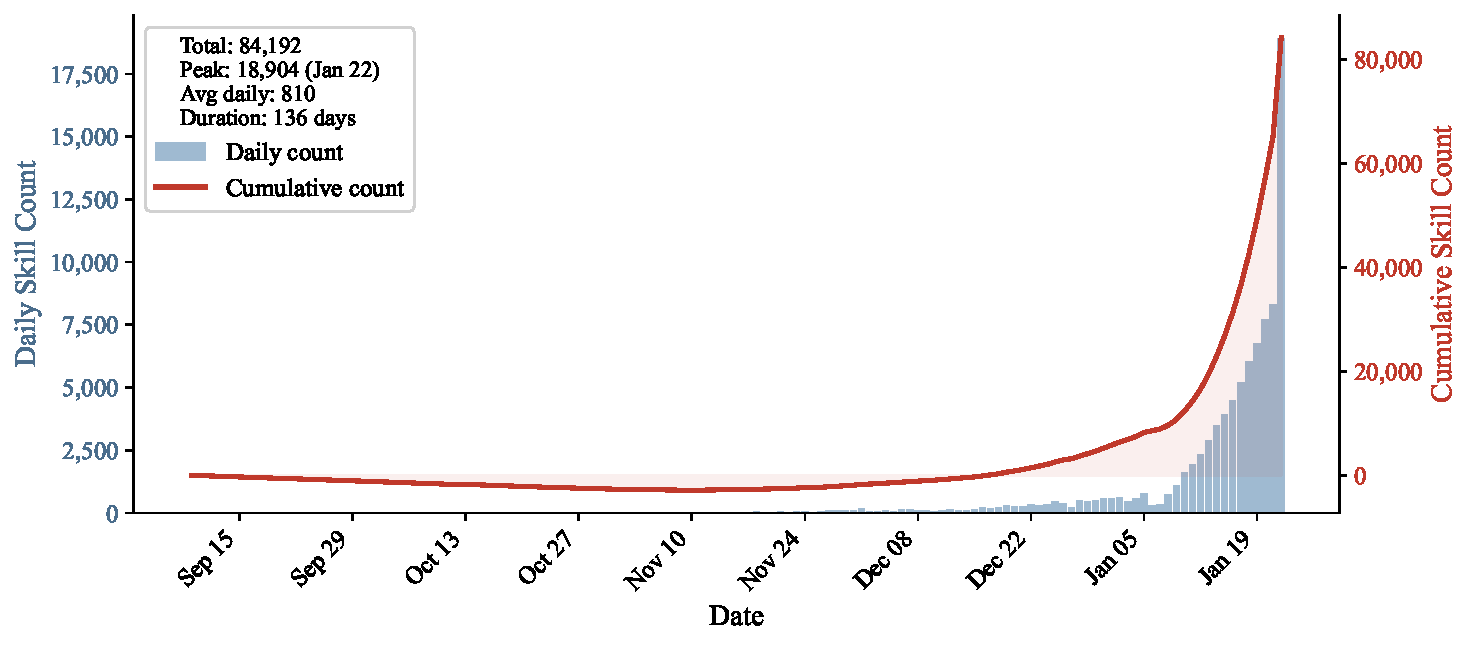
\includegraphics[width=0.8\columnwidth]{figs/figure_timeline_single.pdf}}
    \caption{Temporal dynamics of Skill creation over 136 days. Daily additions (bars, left axis) remained modest through late 2025, then surged to a peak of 18,904 in January 2026. The cumulative curve (line, right axis) reflects exponential-like growth, reaching 84,192 total Skills.}
    \label{fig:timeline}
  \end{center}
\end{figure}

\subsection{Skill Characteristics}

\paragraph{Size Distribution.}
Skill sizes follow a log-normal distribution with median 2.3 KB (IQR: 0.8--6.1 KB).
The largest Skills (top 1\%) exceed 50 KB and typically include extensive code resources.
\autoref{fig:skill_md_length} shows the SKILL.md token distribution, and \autoref{fig:total_length} shows total Skill size distribution.

\begin{figure}[htb]
  \begin{center}
    \centerline{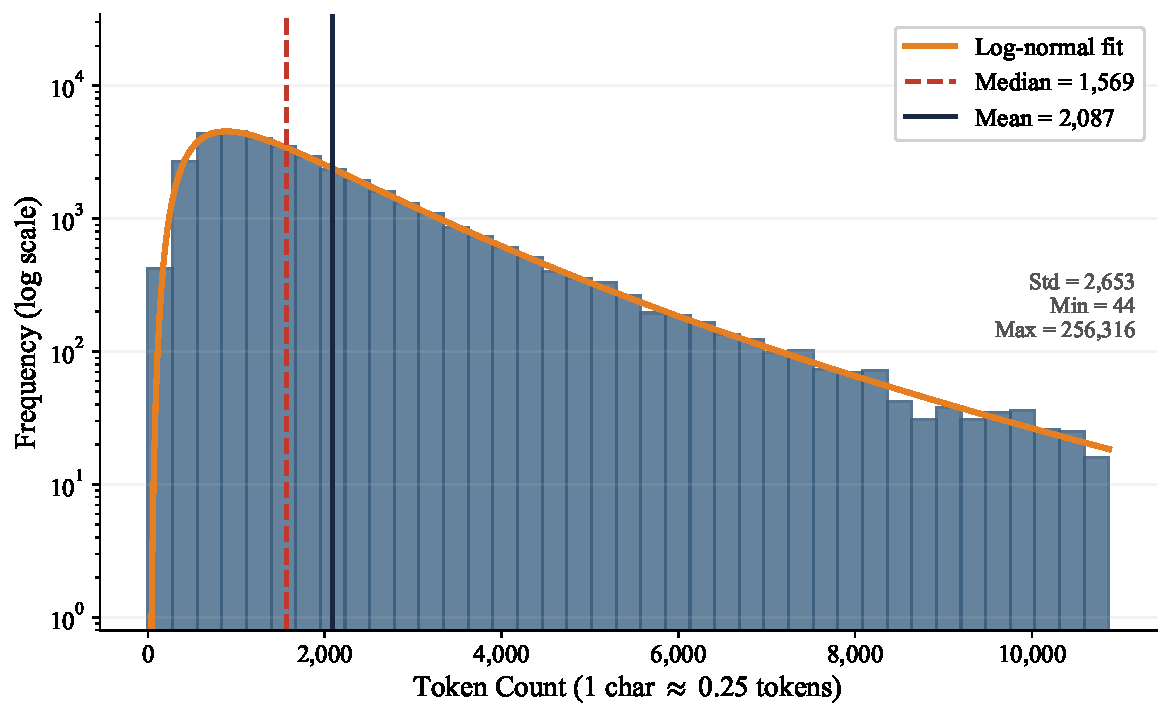
\includegraphics[width=0.8\columnwidth]{figs/figure1_skillmd_distribution.pdf}}
    \caption{Token distribution of SKILL.md files (n=36,338, 99.5th percentile shown). Most Skills are lightweight with median $\sim$1.5k tokens.}
    \label{fig:skill_md_length}
  \end{center}
\end{figure}

\begin{figure}[htb]
  \begin{center}
    \centerline{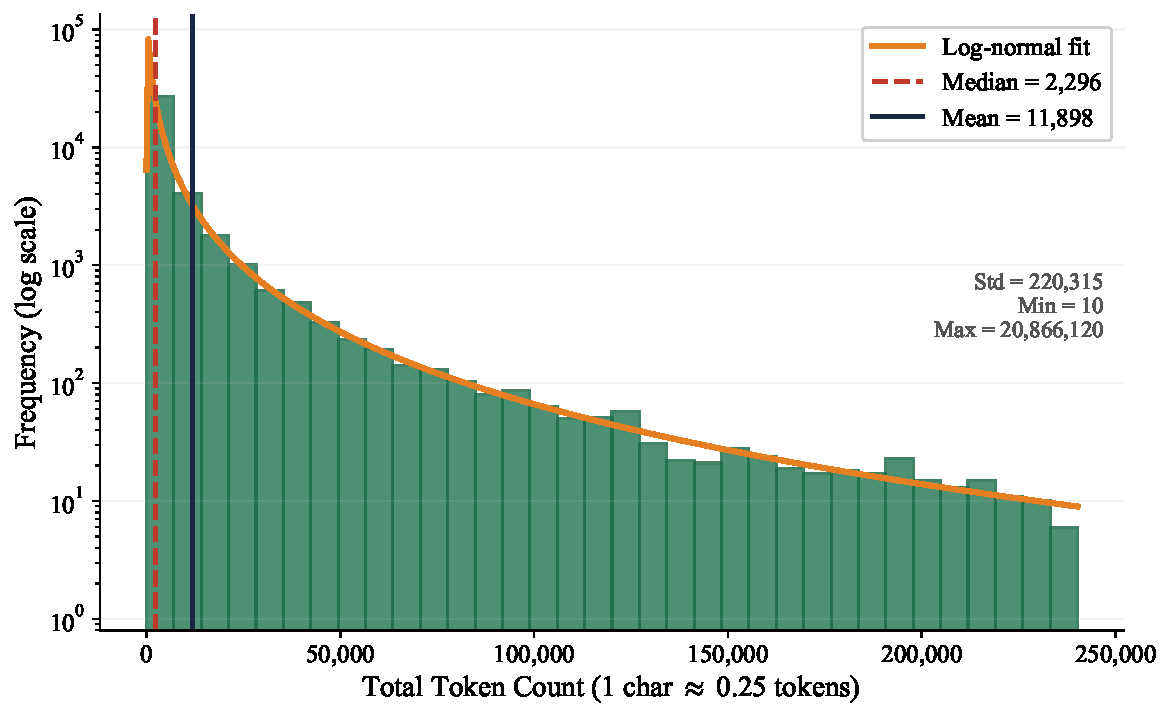
\includegraphics[width=0.8\columnwidth]{figs/figure2_total_distribution.pdf}}
    \caption{Total Skill size distribution (n=37,078, 99.5th percentile shown, excluding metadata.json). Median total size remains under 2.5k tokens, with distribution highly skewed toward concise artifacts.}
    \label{fig:total_length}
  \end{center}
\end{figure}

\paragraph{Domain Coverage.}
Skills span diverse domains (\autoref{fig:category}):
\begin{itemize}[nosep]
    \item Software Development: 38\% (git workflows, code review, testing)
    \item Data Analysis: 22\% (pandas, SQL, visualization)
    \item DevOps/Infrastructure: 15\% (Docker, Kubernetes, CI/CD)
    \item Writing/Documentation: 12\% (technical writing, API docs)
    \item Other: 13\% (scientific computing, finance, etc.)
\end{itemize}

% \begin{figure}[H]
%   \vskip 0.1in
%   \begin{center}
%     \centerline{\includegraphics[width=0.8\columnwidth]{figs/category.png}}
%     \caption{Category distribution of Skills. No single category dominates; Skills are spread across documentation, version control, code quality, CLI tools, DevOps, APIs, and frontend tasks.}
%     \label{fig:category}
%   \end{center}
%   \vskip -0.1in
% \end{figure}

\begin{figure}[htb]
  \begin{center}
    \centerline{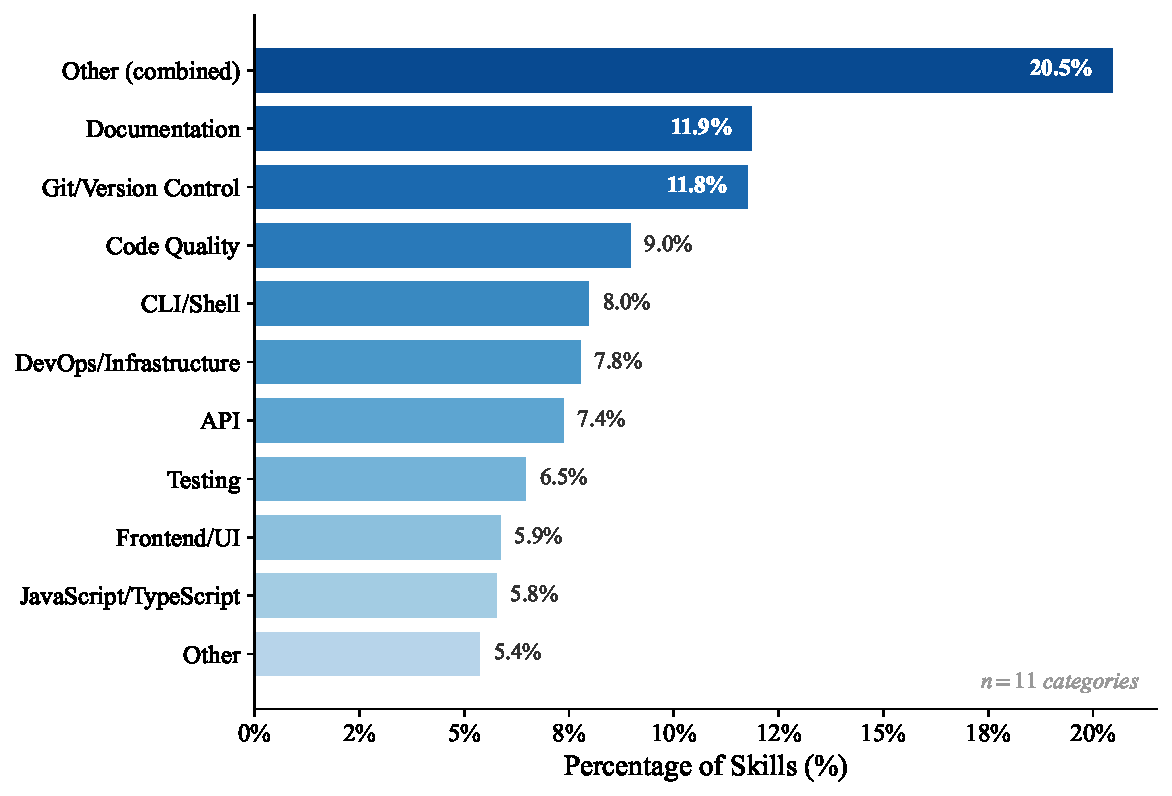
\includegraphics[width=0.7\columnwidth]{figs/categories_gradient.pdf}}
    \caption{Distribution of Skill categories. The top 10 categories account for 79.6\% of all Skills, with Documentation (11.9\%), Git/Version Control (11.8\%), and Code Quality (9.0\%) leading. No single category dominates, reflecting diverse developer needs across documentation, infrastructure, testing, and frontend tasks.}
    \label{fig:category}
  \end{center}
\end{figure}

\paragraph{Structural Patterns.}
Most Skills (78\%) follow the standard structure with SKILL.md plus optional resources.
\autoref{fig:file_count} shows that most Skills contain very few files (median of one, concentrated below five). \autoref{fig:file_extension} confirms the ecosystem is documentation-heavy: markdown files dominate, followed by scripting and configuration code.

\begin{figure}[htb]
  \begin{center}
    \centerline{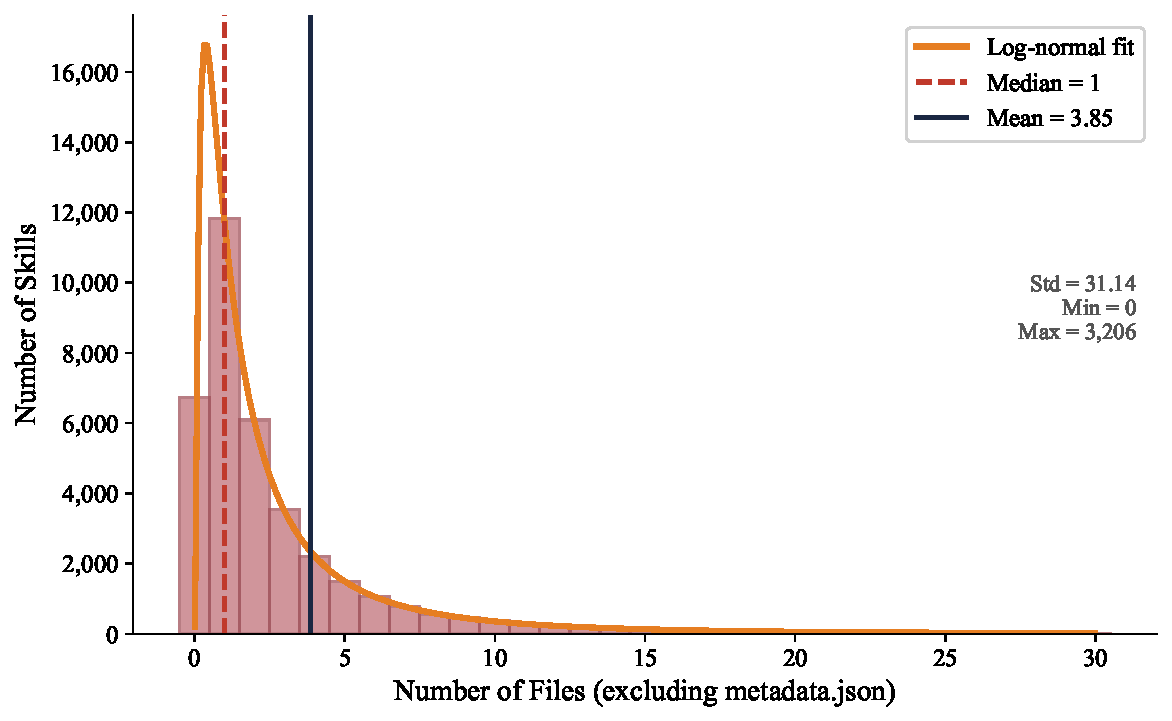
\includegraphics[width=0.8\columnwidth]{figs/figure_file_count.pdf}}
    \caption{File count distribution per Skill. Most Skills contain 1--5 files.}
    \label{fig:file_count}
  \end{center}
\end{figure}

\begin{figure}[htb]
  \begin{center}
    \centerline{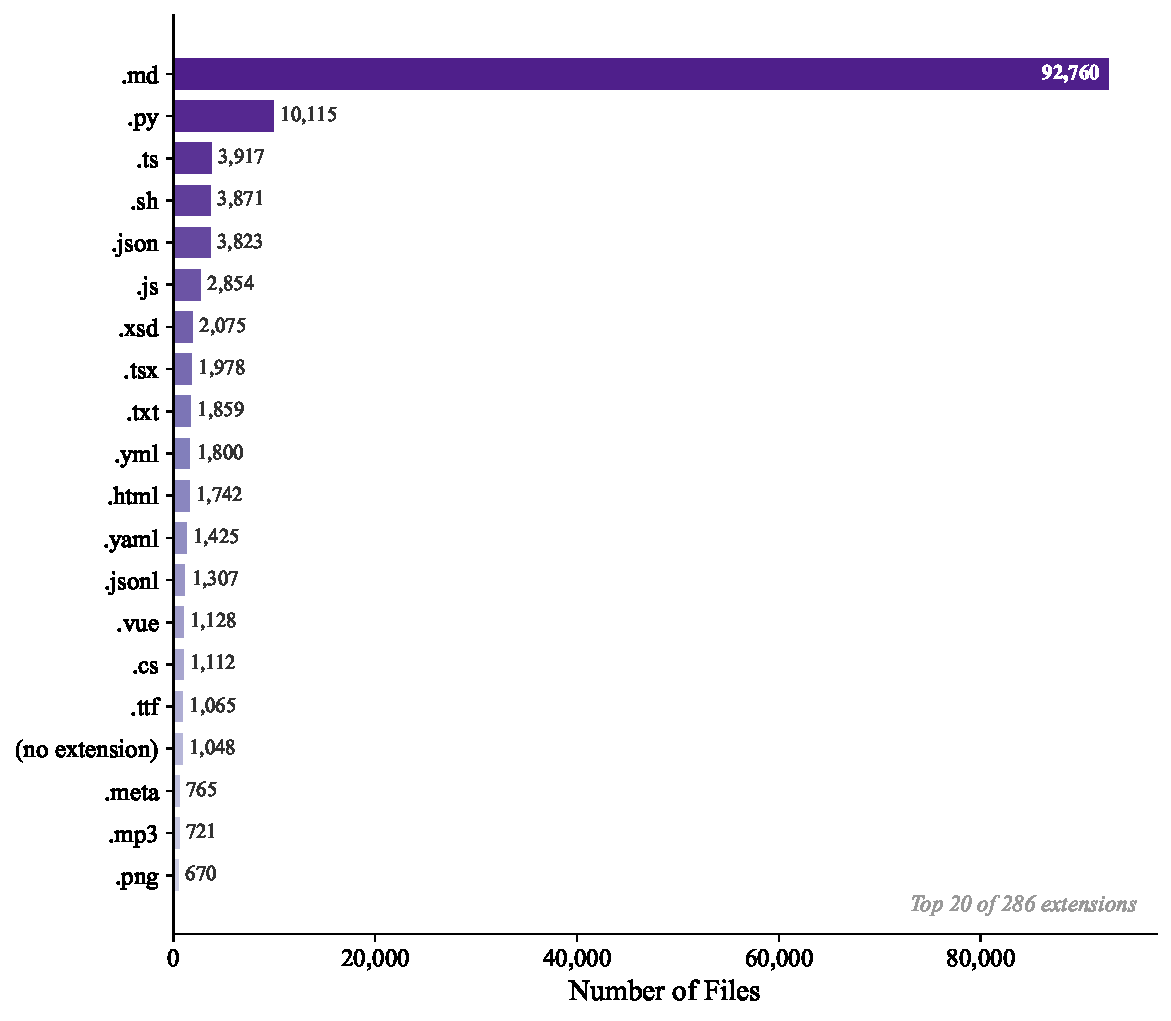
\includegraphics[width=0.8\columnwidth]{figs/extensions_gradient.pdf}}
    \caption{File extension distribution. Markdown files dominate, indicating Skills prioritize natural-language instructions over executable implementations.}
    \label{fig:file_extension}
  \end{center}
\end{figure}

\subsection{Quality Indicators}

We developed a quality scoring rubric based on:
\begin{enumerate}[nosep]
    \item \textbf{Completeness:} Presence of required components (0--3 points)
    \item \textbf{Clarity:} Readability and organization (0--3 points)
    \item \textbf{Specificity:} Actionable vs.\ vague guidance (0--3 points)
    \item \textbf{Examples:} Presence and quality of examples (0--3 points)
\end{enumerate}

Mean quality score across the ecosystem is 6.2/12 (SD=2.8), indicating substantial room for improvement in Skill authoring practices.

\subsection{Implications for Benchmark Design}

This ecosystem analysis directly informed \benchmarkName{} construction:
\begin{itemize}[nosep]
    \item \textbf{Domain selection:} Task categories mirror ecosystem coverage, ensuring Skills exist for evaluation
    \item \textbf{Quality awareness:} Ecosystem mean quality of 6.2/12 motivated our leakage audit and authoring guidelines---low-quality Skills would confound efficacy measurement
    \item \textbf{Skill selection:} We selected benchmark Skills from the top quality quartile (score $\geq$ 9/12) to isolate the effect of procedural knowledge from Skill quality variance
    \item \textbf{Size constraints:} Median Skill size ($\sim$800 tokens) informed our 8K context budget allocation
\end{itemize}

\paragraph{Limitation: Benchmark vs.\ Ecosystem Gap.}
Our 84 evaluated tasks with high-quality Skills represent an optimistic scenario.
Real-world Skill usage involves lower-quality Skills (ecosystem mean: 6.2/12 vs.\ benchmark mean: 10.1/12) and imperfect Skill-task matching.
Future work should evaluate with ecosystem-representative Skill samples.


\section{Task Specification and Review Process}
\label{app:task-spec}

This appendix provides full details of the task specification format and quality control process summarized in \S\ref{sec:SkillsBench}.

\subsection{Task Directory Structure}

Each task is a self-contained directory with the following layout:

\begin{lstlisting}[basicstyle=\footnotesize\ttfamily]
tasks/<task-id>/
  instruction.md          # Task instructions for the agent
  task.toml               # Metadata and resource configuration
  environment/
    Dockerfile            # Container setup
    skills/               # Curated Skills (absent in no-Skills)
      <skill-name>/
        SKILL.md          # Required per skill
        scripts/          # Optional executable code
        references/       # Optional reference documentation
  solution/
    solve.sh              # Oracle solution (must pass 100%)
  tests/
    test.sh               # Runs pytest inside the container
    test_outputs.py       # Programmatic assertions
\end{lstlisting}

\subsection{Task Configuration (\texttt{task.toml})}

Each task specifies metadata and resource limits in TOML format:

\begin{lstlisting}[basicstyle=\footnotesize\ttfamily]
version = "1.0"

[metadata]
author_name = "Contributor Name"
author_email = "email@example.com"
difficulty = "medium"     # easy | medium | hard
category = "finance"
tags = ["pandas", "data-analysis", "spreadsheet"]

[verifier]
timeout_sec = 900.0       # 600-900s typical

[agent]
timeout_sec = 900.0       # 600-1200s typical

[environment]
build_timeout_sec = 600.0
cpus = 1                  # 1-4 cores
memory_mb = 4096          # 2048-10240 MB
storage_mb = 10240        # 10 GB standard
\end{lstlisting}

\subsection{Verification Infrastructure}

Verification uses pytest with the CTRF (Common Test Report Format) output. The \texttt{test.sh} script installs dependencies, runs pytest, and writes a binary reward:

\begin{lstlisting}[language=bash,basicstyle=\footnotesize\ttfamily]
#!/bin/bash
pip3 install --break-system-packages pytest pytest-json-ctrf
mkdir -p /logs/verifier
pytest --ctrf /logs/verifier/ctrf.json \
       /tests/test_outputs.py -rA -v
if [ $? -eq 0 ]; then
  echo 1 > /logs/verifier/reward.txt
else
  echo 0 > /logs/verifier/reward.txt
fi
exit 0
\end{lstlisting}

\noindent A task passes if and only if all assertions in \texttt{test\_outputs.py} succeed (reward = 1). Partial credit is not awarded in the main evaluation.

\subsection{PR Review Process}

Each submitted task undergoes a multi-stage review:
\begin{enumerate}[nosep]
\item \textbf{Automated CI}: Structural validation (\texttt{harbor tasks check}), oracle execution (\texttt{harbor run -a oracle}, must pass 100\%), and AI-detection screening (GPTZero) on \texttt{instruction.md}.
\item \textbf{Maintainer review}: Evaluates data validity, task realism, oracle quality, Skill quality, and anti-cheating robustness. Reviewers run benchmark experiments with and without Skills across multiple agents.
\item \textbf{Benchmark report}: For each task, reviewers produce a structured report documenting oracle results, agent pass rates with and without Skills, failure analysis, and a final verdict (approve, major changes needed, or reject).
\end{enumerate}

\noindent Of 322 candidate submissions from 105 contributors, 86 tasks passed all review stages and were included in the final benchmark (26.7\% acceptance rate).

\subsection{Contributor Checklist}

All task submissions must satisfy the following requirements before review:
\begin{itemize}[nosep]
\item[$\square$] \texttt{instruction.md} is human-written (not model-generated); verified via GPTZero and human review
\item[$\square$] Skills are error-free, factually correct, and generalizable to similar tasks
\item[$\square$] Task is realistic and grounded in professional workflows
\item[$\square$] Task requires domain knowledge and is significantly easier with Skills
\item[$\square$] Outputs are deterministic and verifiable with programmatic assertions
\item[$\square$] Test count is below 10 unless justified; tests cover distinct criteria
\item[$\square$] Oracle solution passes 100\% (\texttt{harbor run -a oracle})
\item[$\square$] Task tested with agent both with and without Skills
\end{itemize}

\subsection{Maintainer Review Policy}

Maintainers evaluate each submission against seven criteria:
\begin{enumerate}[nosep]
\item \textbf{AI detection}: Verify \texttt{instruction.md} and \texttt{task.toml} are manually written using GPTZero and human review. PRs with intentional grammar errors designed to circumvent AI detectors are closed.
\item \textbf{Data quality}: Data must be real-world and appropriately complex. AI-generated or toy data is rejected.
\item \textbf{Task validity}: Tasks must be grounded in realistic professional scenarios. Artificially inflated complexity is rejected.
\item \textbf{Oracle quality}: Simple solutions (e.g., an Excel formula or short script) are preferred over over-engineered oracle implementations.
\item \textbf{Author history}: Authors flagged multiple times across PRs are closed automatically.
\item \textbf{Test parsimony}: Fewer than 10 test cases unless justified; tests should cover distinct criteria rather than repeat similar checks.
\item \textbf{Multimodal verification}: For multimodal tasks (audio, PPTX, video, PDF), maintainers personally inspect agent output to verify correctness beyond programmatic assertions.
\end{enumerate}

\subsection{Automated CI Pipeline}

The CI pipeline performs the following checks on each PR:
\begin{itemize}[nosep]
\item \textbf{Structural validation} (\texttt{harbor tasks check}): Verifies required files exist, TOML schema is valid, Dockerfile builds, and test structure is correct.
\item \textbf{Oracle execution} (\texttt{harbor run -a oracle}): Runs the oracle solution end-to-end and requires 100\% test pass rate.
\item \textbf{AI-detection screening}: Runs GPTZero on \texttt{instruction.md} to flag potential model-generated content.
\item \textbf{LLM-backed quality checks}: Automated verification of behavior consistency between instructions and tests, anti-cheating measures, pinned dependency checks, typo detection, and hardcoded solution detection.
\end{itemize}

\subsection{Benchmark Report Template}

For each task, reviewers produce a structured report documenting:
\begin{enumerate}[nosep]
\item \textbf{Task metadata}: Name, category, difficulty, tags, description, Skills provided, key requirements.
\item \textbf{Oracle results}: Pass/fail status, reward, tests passed, timing.
\item \textbf{Agent results}: Pass rates per agent-model combination, with and without Skills, including execution time.
\item \textbf{Skills impact}: Quantified comparison of with-Skills vs.\ without-Skills performance per agent.
\item \textbf{Failure analysis}: Per-test breakdown of failures including actual vs.\ expected output, root cause, and evidence from trajectories.
\item \textbf{Recommendation}: One of: \textsc{approve}, \textsc{approve with caveats}, \textsc{major changes needed}, or \textsc{reject}.
\end{enumerate}

\subsection{Review Lifecycle}

PRs progress through a defined label-based lifecycle:
\begin{enumerate}[nosep]
\item \textbf{WIP} $\rightarrow$ \textbf{Need review}: Author signals readiness for initial review.
\item \textbf{Need review} $\rightarrow$ \textbf{Reviewing}: A maintainer begins active review and benchmark experiments.
\item \textbf{Reviewing} $\rightarrow$ \textbf{Change requested / Major change needed / Critical change needed}: Issues identified; author must address.
\item \textbf{Change requested} $\rightarrow$ \textbf{Take another look}: Author responds after changes.
\item \textbf{Ready to merge} $\rightarrow$ \textbf{Good task}: All reviews passed; task included in benchmark.
\end{enumerate}

\noindent Critical changes include unrealistic task scenarios, AI-generated instructions, or synthetic data. Major changes include incorrect tests, unreliable verifiers, or poor Skill quality requiring re-evaluation.

\subsection{Task Quality Criteria}

Tasks are evaluated against the following criteria:
\begin{itemize}[nosep]
\item \textbf{Realistic}: Grounded in professional workflows that people in that domain actually perform
\item \textbf{Skill-dependent}: Significantly easier with Skills than without---tasks solvable without any procedural guidance are rejected
\item \textbf{Verifiable}: Deterministic outputs testable with programmatic assertions; LLM-as-judge is not used
\item \textbf{Composable}: Tasks should exercise 3--6 Skills together; instructions never reference which Skills to use
\item \textbf{Test parsimony}: Fewer than 10 test cases unless justified; tests should cover distinct criteria rather than repeat similar checks
\end{itemize}


\section{Experimental Setup Details}
\label{app:exp-details}

This appendix provides full details of the experimental setup summarized in \S\ref{sec:experimentation}.

\subsection{Model and Harness Configurations}

\autoref{tab:models-full} presents all 7 agent-model configurations evaluated in the main experiments.

\begin{table}[htb]
\centering
\footnotesize
\caption{Agent harnesses and models evaluated. Total: 7,308 valid trajectories across 7 configurations and 3 conditions (no Skills, with Skills, self-generated Skills). Self-generated condition evaluated on Claude Code and Codex configurations only.}
\setlength{\tabcolsep}{3pt}
\begin{tabular}{llll}
\toprule
\textbf{Harness} & \textbf{Model} & \textbf{Provider} & \textbf{Runs} \\
\midrule
\multirow{4}{*}{Claude Code} & Opus 4.5 & Anthropic & 1092 \\
& Opus 4.6 & Anthropic & 1260 \\
& Sonnet 4.5 & Anthropic & 1092 \\
& Haiku 4.5 & Anthropic & 1092 \\
\midrule
\multirow{2}{*}{Gemini CLI} & Gemini 3 Pro & Google & 840 \\
& Gemini 3 Flash & Google & 840 \\
\midrule
Codex & GPT-5.2 & OpenAI & 1092 \\
\bottomrule
\end{tabular}

\label{tab:models-full}
\end{table}

\subsection{Harness Descriptions}

We evaluate three commercial agent harnesses:
\begin{itemize}[nosep]
    \item \textbf{Claude Code}~\citep{anthropic2025claudecode}: Anthropic's agent with native Skill integration
    \item \textbf{Gemini CLI}~\citep{google2025geminicli}: Google's open-source terminal agent
    \item \textbf{Codex CLI}~\citep{openai2025codexcli}: OpenAI's lightweight coding agent
\end{itemize}
These tightly couple specific models with proprietary agent logic, representing real-world deployment conditions.

\paragraph{Model Family Consideration.} Claude models have been trained with awareness of the Agent Skills specification~\citep{anthropic2025agentskills}, which may confer advantages when processing Skill-formatted instructions.

\subsection{Agent Interface}

Agents interact with the environment through a standardized interface:

\begin{lstlisting}[language=Python,basicstyle=\footnotesize\ttfamily]
class BaseAgent(ABC):
    @abstractmethod
    def step(self, obs: str) -> str:
        """obs: terminal output -> action"""
        pass
\end{lstlisting}

\subsection{Skill Injection Mechanism}
\label{app:injection}

Skills are injected into each task's Docker container by copying the \texttt{environment/skills/} directory to agent-specific paths. Each Dockerfile includes:

\begin{lstlisting}[language=bash,basicstyle=\footnotesize\ttfamily]
# Copy skills to agent-specific locations
COPY skills /root/.claude/skills    # Claude Code
COPY skills /root/.codex/skills     # Codex CLI
COPY skills /root/.gemini/skills    # Gemini CLI
COPY skills /root/.agents/skills    # Portable agents
\end{lstlisting}

Each agent harness discovers and loads Skills from its respective directory at runtime using its native skill scanning mechanism. Claude Code and Codex read the \texttt{SKILL.md} frontmatter (name and description) to determine relevance; Gemini CLI exposes an \texttt{activate\_skill} tool that agents invoke explicitly. Instructions never reference which Skills to use---agents must discover and apply them autonomously.

\subsection{Skill Structure}

Each Skill is a directory containing a required \texttt{SKILL.md} file with YAML frontmatter and optional bundled resources:

\begin{lstlisting}[basicstyle=\footnotesize\ttfamily]
skill-name/
  SKILL.md          # Required: YAML frontmatter + instructions
  scripts/          # Optional: executable code
  references/       # Optional: reference documentation
\end{lstlisting}

\noindent The \texttt{SKILL.md} frontmatter specifies the Skill's name and a one-line description used by agents for skill discovery. The body contains procedural guidance, code examples, and usage patterns.

\subsection{Self-Generated Skills Condition}
\label{app:self-gen}

For the self-generated condition, tasks are identical to the no-Skills baseline except that the following prompt is appended to each \texttt{instruction.md}:

\begin{quote}
\small
\textbf{Important: Generate Skills First}

Before attempting to solve this task, please follow these steps:

\begin{enumerate}[nosep]
\item Analyze the task requirements and identify what domain knowledge, APIs, or techniques are needed.
\item Write 1--5 modular skill documents that would help solve this task. Each skill should:
  focus on a specific tool, library, API, or technique;
  include installation/setup instructions if applicable;
  provide code examples and usage patterns;
  be reusable for similar tasks.
\item Save each skill as a markdown file in the \texttt{environment/skills/} directory with a descriptive name.
\item Then solve the task using the skills you created as reference.
\end{enumerate}
\end{quote}

\noindent The \texttt{environment/skills/} directory is empty at the start---agents must populate it before solving the task. No curated Skills are provided. The self-generated condition is evaluated on Claude Code (all four models) and Codex (GPT-5.2) only; Gemini CLI does not support this condition due to its explicit skill-activation interface.

\subsection{Software and Model Versions}

\autoref{tab:versions} lists the exact model identifiers and harness versions used in all experiments.

\begin{table}[htb]
\centering
\footnotesize
\caption{Model API identifiers and harness versions.}
\label{tab:versions}
\begin{tabular}{lll}
\toprule
\textbf{Display Name} & \textbf{API Model ID} & \textbf{Harness Version} \\
\midrule
Claude Opus 4.5 & \texttt{claude-opus-4-5@20251101} & Claude Code 2.1.19 \\
Claude Opus 4.6 & \texttt{claude-opus-4-6} & Claude Code 2.1.19 \\
Claude Sonnet 4.5 & \texttt{claude-sonnet-4-5@20250929} & Claude Code 2.1.19 \\
Claude Haiku 4.5 & \texttt{claude-haiku-4-5@20251001} & Claude Code 2.1.19 \\
GPT-5.2 & \texttt{openai/gpt-5.2-codex} & Codex CLI \\
Gemini 3 Pro & \texttt{gemini/gemini-3-pro-preview} & Gemini CLI \\
Gemini 3 Flash & \texttt{gemini/gemini-3-flash-preview} & Gemini CLI \\
\bottomrule
\end{tabular}
\end{table}

\subsection{Container Environment}

All tasks run in Docker containers built from an \texttt{ubuntu:24.04} base image. Per-task resource allocation is specified in \texttt{task.toml}:

\begin{itemize}[nosep]
    \item \textbf{CPUs}: 1--4 cores (task-dependent)
    \item \textbf{Memory}: 2--10 GB (task-dependent)
    \item \textbf{Storage}: 10 GB (standard across all tasks)
    \item \textbf{GPU}: None (no tasks require GPU)
\end{itemize}

\noindent Containers are deleted after each trial (\texttt{delete: true}) to ensure no state leaks between runs.

\subsection{Inference Configuration}

\begin{itemize}[nosep]
    \item \textbf{Temperature}: 0 (deterministic sampling)
    \item \textbf{Max rounds}: Level-dependent (10/30/50 for Core/Extended/Extreme)
    \item \textbf{Context management}: Sliding window with 8K token limit; oldest turns dropped when exceeded
    \item \textbf{Timeout}: Per-task, specified in \texttt{task.toml} (range: 600--1200s)
\end{itemize}

\subsection{Experiment Orchestration}

\begin{itemize}[nosep]
    \item \textbf{Runs per task}: 5 for main conditions (no Skills, with Skills); 3 for self-generated condition
    \item \textbf{Concurrent trials}: 256 (main conditions); 128 (self-generated)
    \item \textbf{Retry policy}: No retries for main conditions; up to 3 retries for self-generated (excluding \texttt{VerifierTimeoutError}, \texttt{BadRequestError}, \texttt{RateLimitError}, \texttt{AgentTimeoutError})
    \item \textbf{Excluded tasks}: \texttt{mhc-layer-impl} (GPU requirement) and \texttt{fix-visual-stability} (verifier timeout) are excluded from all experiments
\end{itemize}

\noindent The evaluation comprises 7,308 valid trajectories across 7 configurations, 84 tasks, and 3 conditions. We report mean pass rates with 95\% bootstrap confidence intervals.



\section{Task-Level Results}
\label{app:task-level}

\autoref{fig:heatmap-with}, \autoref{fig:heatmap-no}, and \autoref{fig:heatmap-uplift} show the task-level pass rates per model across all 84 evaluated tasks.
Results are averaged over 5 trials per task-model-condition combination.
Tasks (rows) are sorted by average with-Skills pass rate; models (columns) are sorted by aggregate with-Skills score.

\begin{figure}[p]
  \begin{center}
    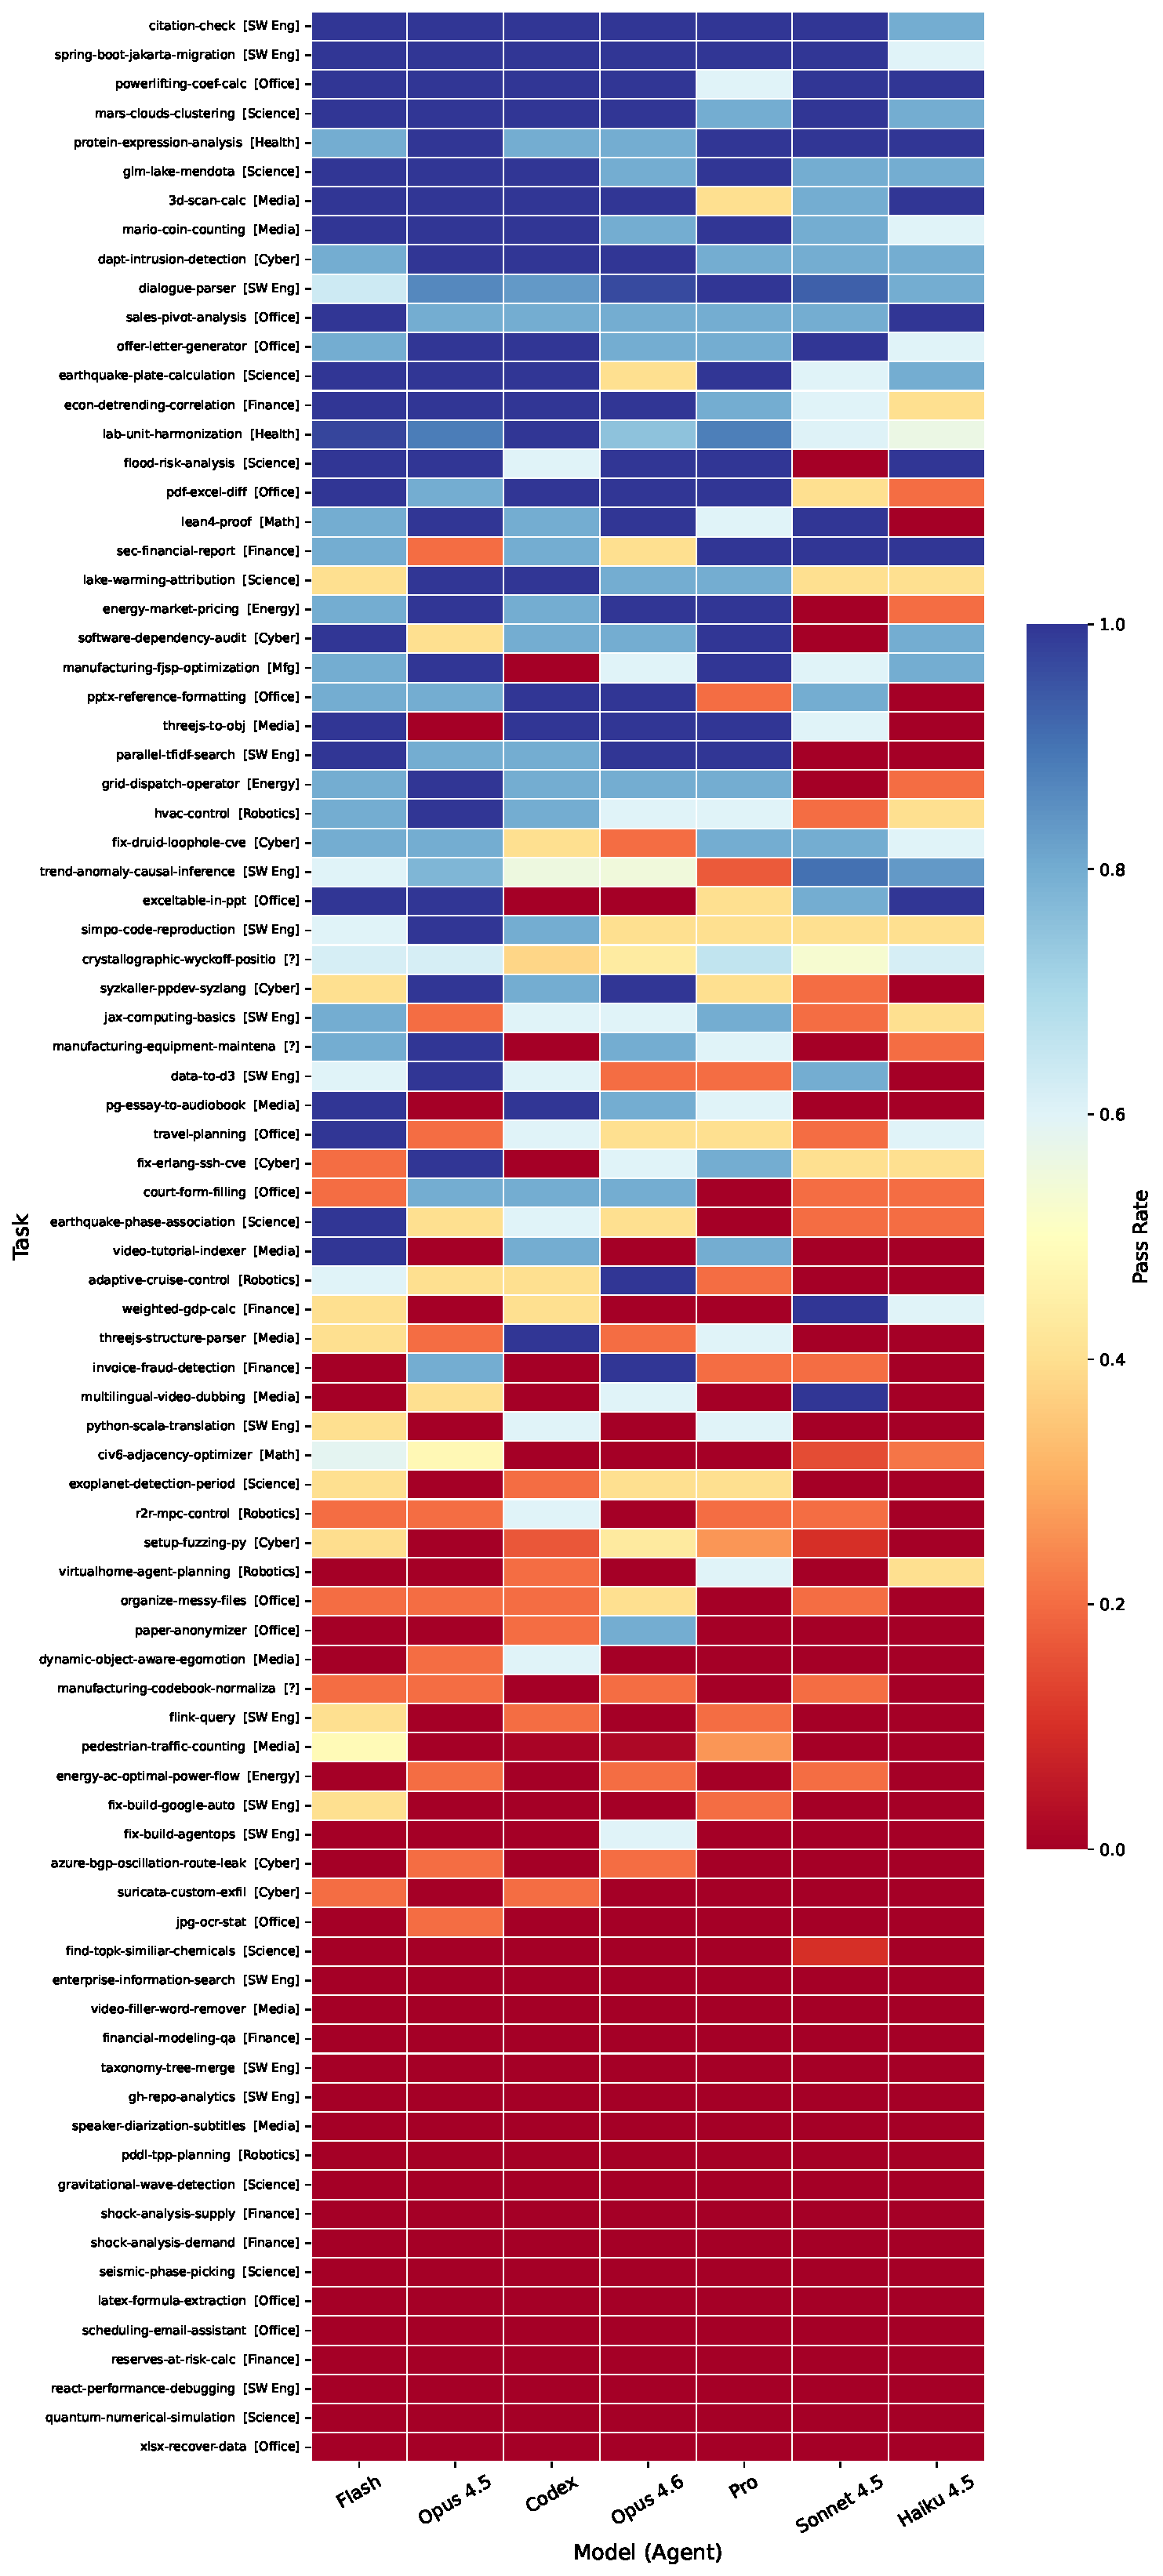
\includegraphics[width=\textwidth,height=0.88\textheight,keepaspectratio]{figs/heatmap_with_skills.pdf}
    \caption{Task pass rate per model with curated Skills. The grid reveals a common set of easy tasks (top, uniformly blue) solved by all models, and hard tasks (bottom, uniformly red) unsolved even with Skills. Tasks along the diagonal transition from solvable to unsolvable as model capability decreases.}
    \label{fig:heatmap-with}
  \end{center}
\end{figure}

\begin{figure}[p]
  \begin{center}
    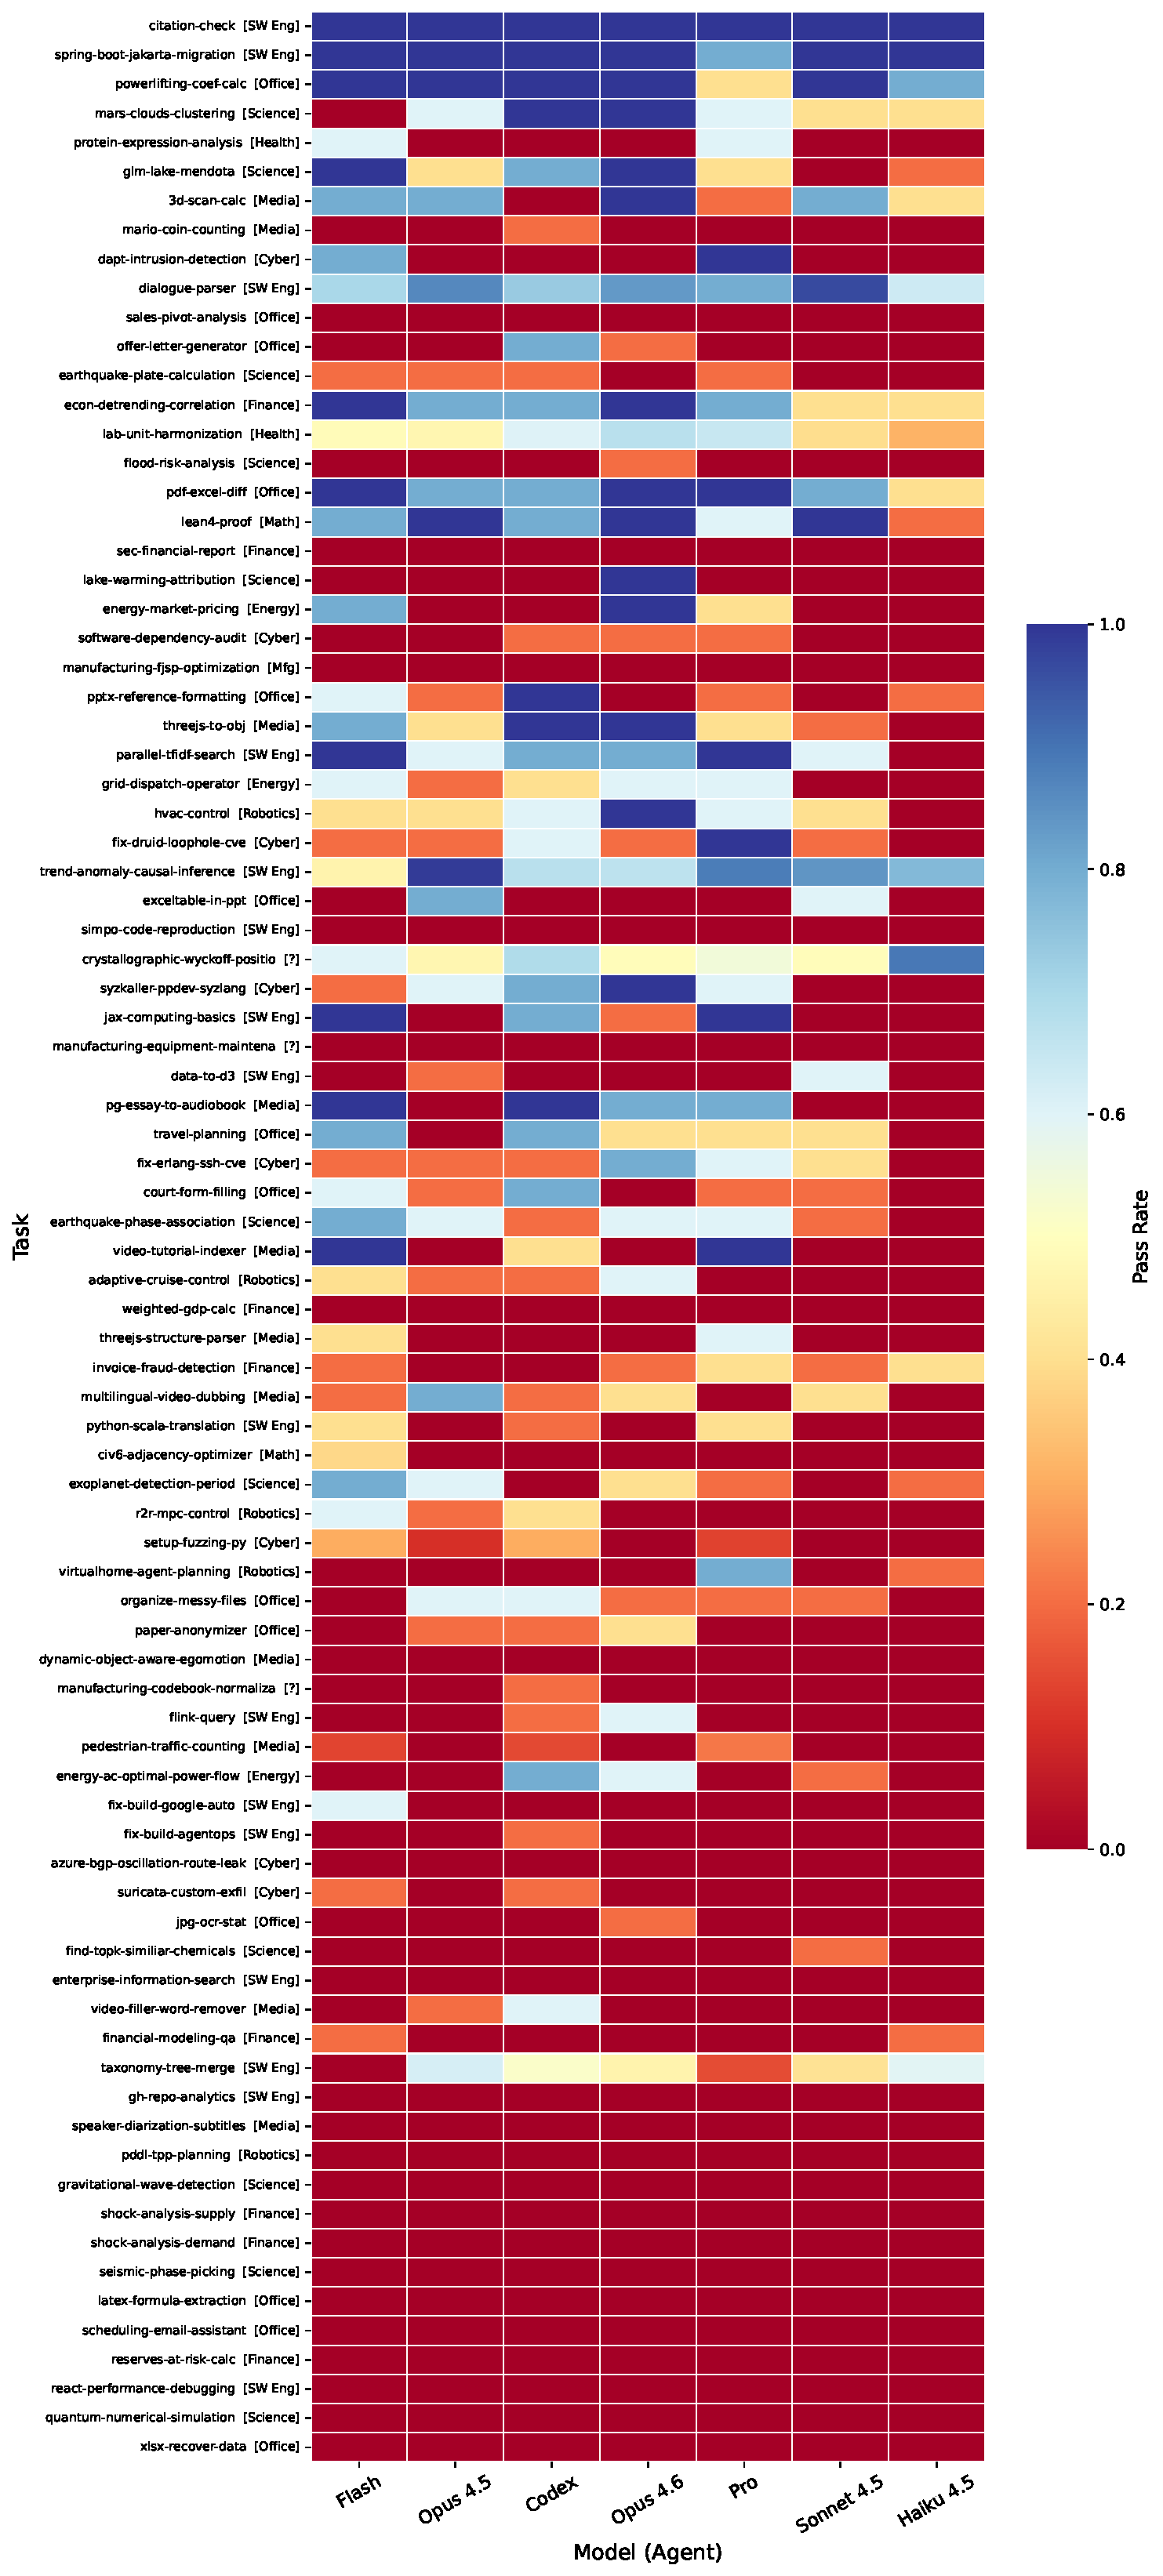
\includegraphics[width=\textwidth,height=0.88\textheight,keepaspectratio]{figs/heatmap_no_skills.pdf}
    \caption{Task pass rate per model without Skills (baseline). Compared to \autoref{fig:heatmap-with}, the blue region contracts substantially, confirming that Skills shift many tasks from unsolved to solved.}
    \label{fig:heatmap-no}
  \end{center}
\end{figure}

\begin{figure}[p]
  \begin{center}
    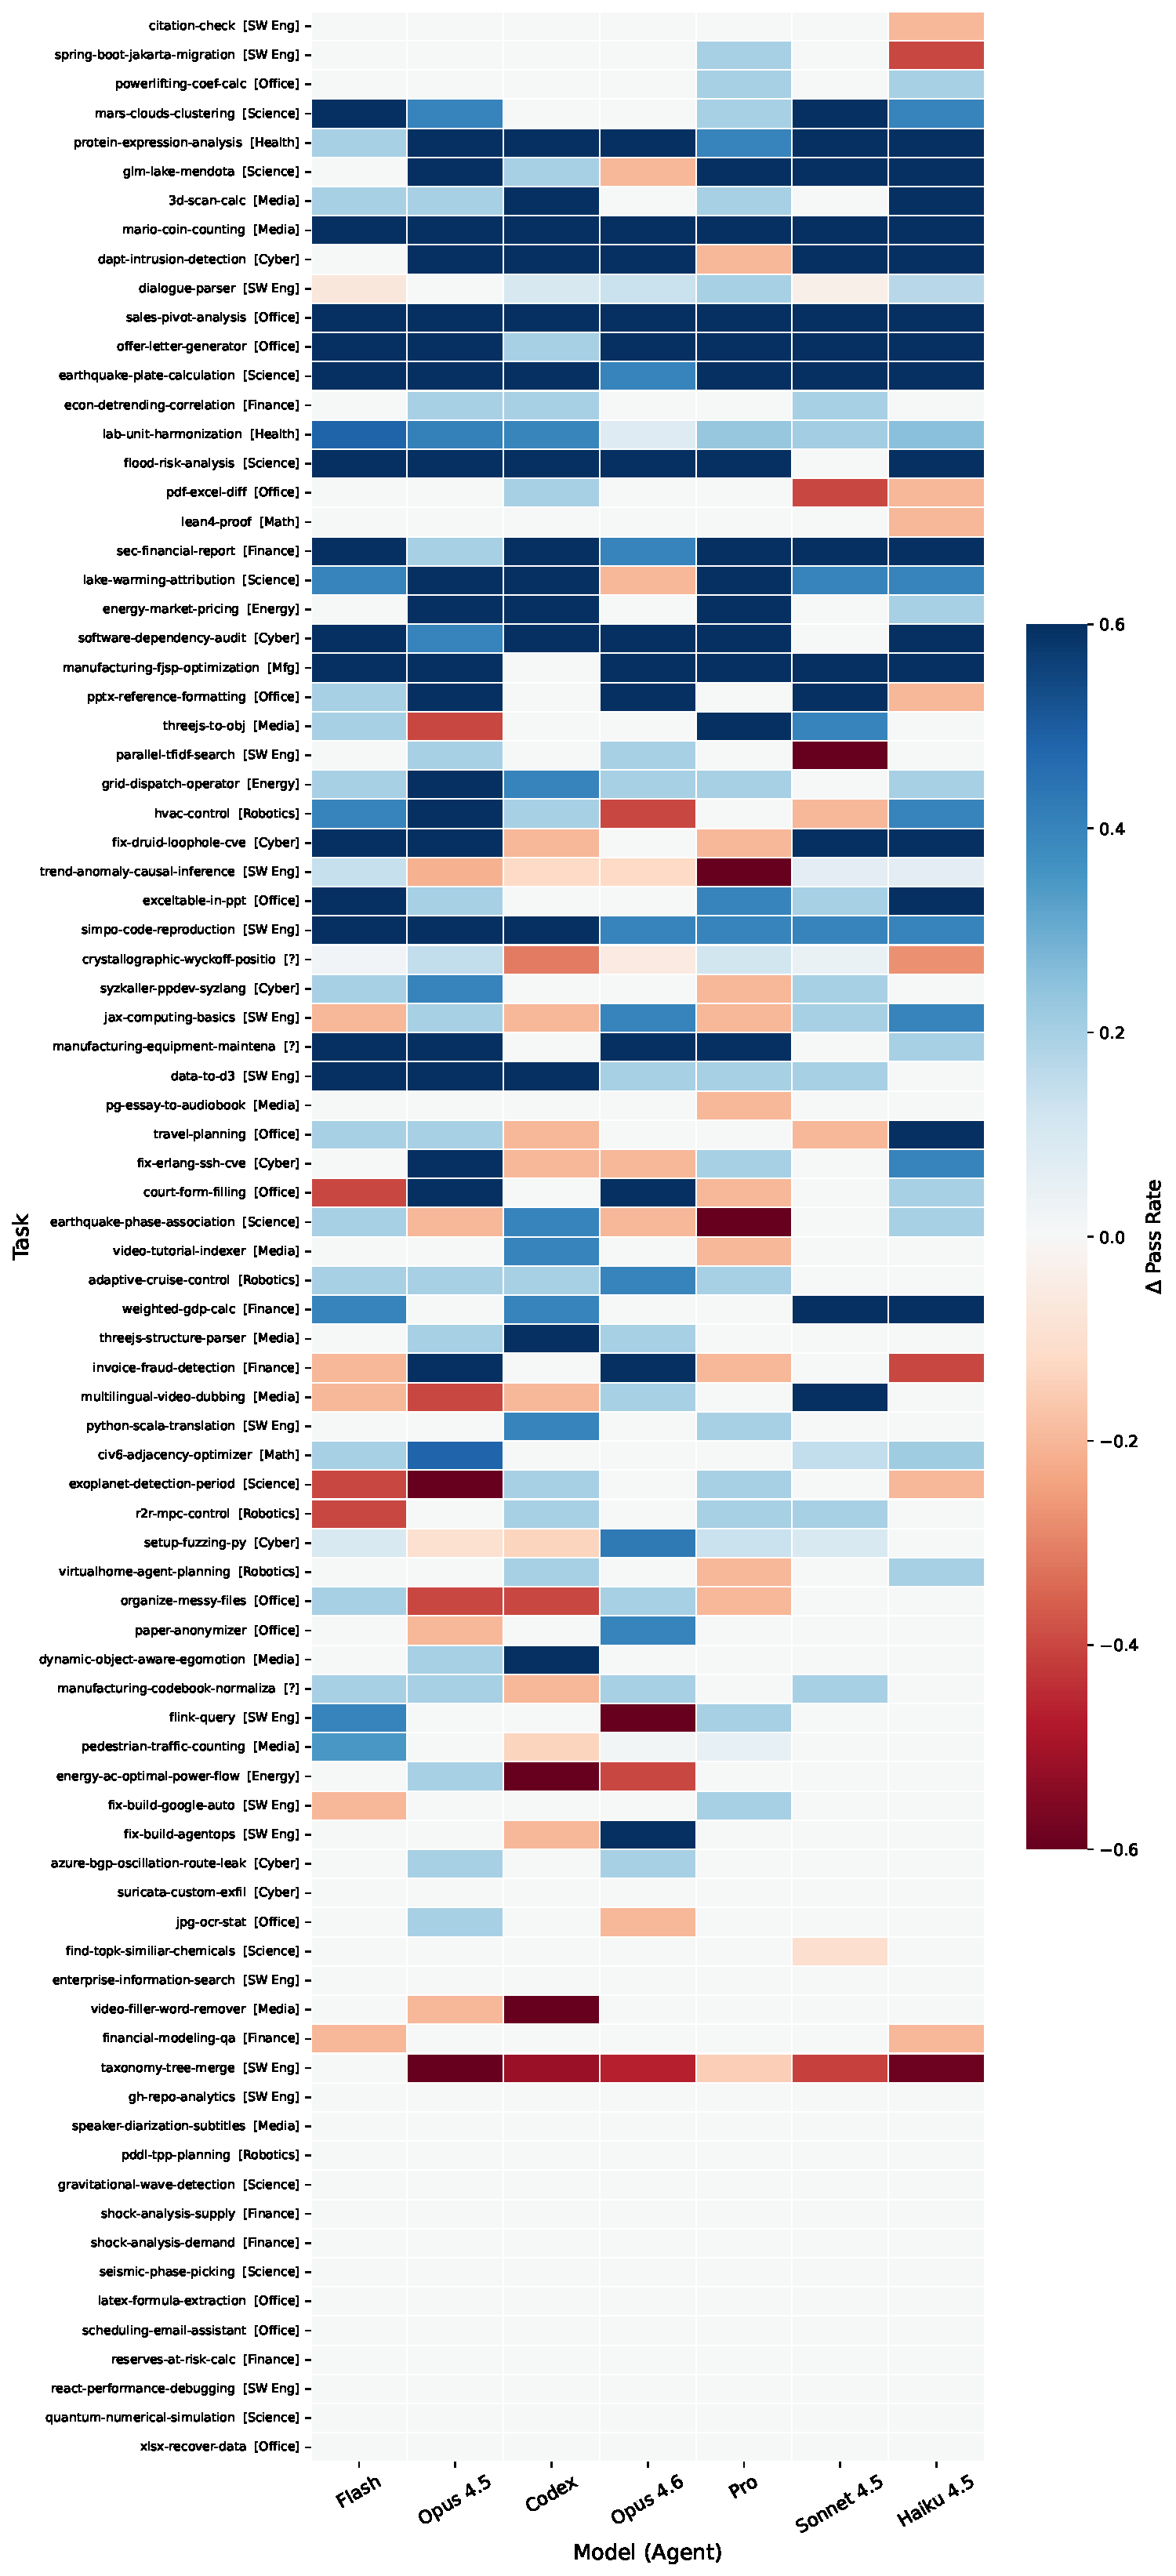
\includegraphics[width=\textwidth,height=0.88\textheight,keepaspectratio]{figs/heatmap_skills_uplift.pdf}
    \caption{Skills uplift per task (with Skills $-$ without Skills). Blue cells indicate positive uplift; red cells indicate tasks where Skills hurt performance. The majority of cells are blue, confirming broad Skill benefit. A small number of tasks show negative delta for specific models.}
    \label{fig:heatmap-uplift}
  \end{center}
\end{figure}


\section{Additional Experimental Details}
\label{app:details}

\subsection{Confidence Interval Calculation}

We compute 95\% confidence intervals using the percentile bootstrap method with 1,000 resamples.
For normalized gain, we compute CIs on the gain metric directly rather than on the component pass rates.

\subsection{10-Run Validation}

For a subset of configurations (GPT-5.2 and Claude Opus 4.5, all 26 Extreme tasks, no-Skills and with-Skills conditions), we conducted 10 runs instead of 5. Results show:
\begin{itemize}[nosep]
    \item Mean $\Delta$ within 1.2pp of 5-run estimates
    \item Standard error reduced by $\sim$30\%
    \item All conclusions remain unchanged
\end{itemize}

This validates that 5 runs provides sufficient precision for our main findings.


% \section{Reproducibility Checklist}
% \label{app:reproducibility}

% \begin{itemize}
%     \item[$\square$] Code and evaluation scripts will be released
%     \item[$\square$] Task specifications with Dockerfiles provided
%     \item[$\square$] All Skills used in evaluation documented
%     \item[$\square$] Model API versions and settings specified
%     \item[$\square$] Random seeds and determinism settings documented
%     \item[$\square$] Complete results tables in supplementary materials
% \end{itemize}

\section{Complete Task List}
\label{app:task-list}

\autoref{tab:task-list} enumerates all 86 tasks in \benchmarkName{}, organized by domain. Two tasks are excluded from evaluation: \texttt{mhc-layer-impl} (requires GPU) and \texttt{fix-visual-stability} (verifier timeout), leaving 84 evaluated tasks. Difficulty levels are assigned by task authors and validated during review.

\footnotesize
\begin{longtable}{p{4.5cm}p{2.5cm}cp{7.5cm}}
\caption{Complete list of \benchmarkName{} tasks (86 total, 84 evaluated). Tasks are grouped by domain and sorted alphabetically within each domain.} \label{tab:task-list} \\
\toprule
\textbf{Task ID} & \textbf{Domain} & \textbf{Diff.} & \textbf{Description} \\
\midrule
\endfirsthead

\multicolumn{4}{c}{\footnotesize\tablename\ \thetable\ -- continued from previous page} \\
\toprule
\textbf{Task ID} & \textbf{Domain} & \textbf{Diff.} & \textbf{Description} \\
\midrule
\endhead

\midrule
\multicolumn{4}{r}{\footnotesize Continued on next page} \\
\endfoot

\bottomrule
\endlastfoot

% --- Cybersecurity (8) ---
\texttt{azure-bgp-oscillation} & Cybersecurity & Med & Detect BGP route oscillation and leaks in Azure Virtual WAN topology \\
\texttt{dapt-intrusion-detection} & Cybersecurity & Hard & Compute network statistics from PCAP file (DAPT2020 traffic) \\
\texttt{fix-druid-loophole-cve} & Cybersecurity & Hard & Fix Apache Druid 0.20.0 arbitrary code execution vulnerability \\
\texttt{fix-erlang-ssh-cve} & Cybersecurity & Hard & Fix Erlang/OTP SSH server unauthenticated RCE vulnerability \\
\texttt{setup-fuzzing-py} & Cybersecurity & Med & Set up continuous fuzzing for 5 Python libraries \\
\texttt{software-dependency-audit} & Cybersecurity & Med & Security audit of npm dependencies for vulnerabilities \\
\texttt{suricata-custom-exfil} & Cybersecurity & Med & Write Suricata signatures to detect HTTP data exfiltration \\
\texttt{syzkaller-ppdev-syzlang} & Cybersecurity & Med & Write syzkaller syzlang support for Linux parallel port driver \\
\midrule

% --- Energy (3) ---
\texttt{energy-ac-optimal-power} & Energy & Med & Solve AC optimal power flow for day-ahead market schedule \\
\texttt{energy-market-pricing} & Energy & Hard & Analyze congestion pricing with counterfactual transmission relaxation \\
\texttt{grid-dispatch-operator} & Energy & Med & Decide generator dispatches for economically efficient DC power flow \\
\midrule

% --- Finance (8) ---
\texttt{econ-detrending-corr.} & Finance & Med & Calculate Pearson correlation between detrended consumption and investment \\
\texttt{financial-modeling-qa} & Finance & Hard & Analyze large-scale financial data and answer modeling questions \\
\texttt{invoice-fraud-detection} & Finance & Hard & Detect invoice fraud by cross-referencing PDFs, Excel, and CSV \\
\texttt{reserves-at-risk-calc} & Finance & Med & Calculate Reserves-at-Risk using IMF gold price and reserves data \\
\texttt{sec-financial-report} & Finance & Hard & Analyze hedge fund activities comparing Q2 vs Q3 2025 SEC filings \\
\texttt{shock-analysis-demand} & Finance & Med & Estimate investment shock to Georgia (demand-side macro framework) \\
\texttt{shock-analysis-supply} & Finance & Hard & Estimate investment shock to Georgia (Cobb-Douglas production) \\
\texttt{weighted-gdp-calc} & Finance & Med & Calculate weighted mean of GCC net exports as \% of GDP \\
\midrule

% --- Healthcare (2) ---
\texttt{lab-unit-harmonization} & Healthcare & Med & Harmonize clinical lab data units across healthcare systems \\
\texttt{protein-expression-analysis} & Healthcare & Med & Analyze differential protein expression in cancer cell line data \\
\midrule

% --- Manufacturing (3) ---
\texttt{mfg-codebook-norm.} & Manufacturing & Med & Normalize manufacturing defect reason texts to standard codebook \\
\texttt{mfg-equipment-maint.} & Manufacturing & Med & Answer reflow machine maintenance questions from handbook data \\
\texttt{mfg-fjsp-optimization} & Manufacturing & Med & Optimize flexible job shop schedule with downtime constraints \\
\midrule

% --- Mathematics (2) ---
\texttt{civ6-adjacency-optimizer} & Mathematics & Hard & Optimize adjacency bonuses in Civilization 6 district placement \\
\texttt{lean4-proof} & Mathematics & Med & Complete a Lean4 formal proof for a sequence problem \\
\midrule

% --- Media \& Content Production (11) ---
\texttt{3d-scan-calc} & Media \& Content & Hard & Calculate mass of 3D printed part from binary STL file \\
\texttt{dynamic-obj-egomotion} & Media \& Content & Med & Analyze camera egomotion and detect dynamic objects in video \\
\texttt{mario-coin-counting} & Media \& Content & Med & Count coins/enemies/turtles in Super Mario video frames \\
\texttt{multilingual-video-dub} & Media \& Content & Med & Perform multilingual video dubbing with TTS alignment \\
\texttt{pedestrian-traffic-count} & Media \& Content & Hard & Count pedestrians in surveillance camera videos \\
\texttt{pg-essay-to-audiobook} & Media \& Content & Med & Convert Paul Graham essays to audiobook via TTS \\
\texttt{speaker-diarization-subs} & Media \& Content & Hard & Perform speaker diarization and generate subtitles from video \\
\texttt{threejs-structure-parser} & Media \& Content & Med & Parse Three.js file to extract 3D object part-level structure \\
\texttt{threejs-to-obj} & Media \& Content & Med & Convert Three.js 3D object to OBJ format for Blender \\
\texttt{video-filler-word-remover} & Media \& Content & Med & Detect filler words and their timestamps in interview video \\
\texttt{video-tutorial-indexer} & Media \& Content & Hard & Find chapter start timestamps in a 23-min Blender tutorial \\
\midrule

% --- Natural Science (12) ---
\texttt{crystallographic-wyckoff} & Natural Science & Med & Analyze crystal structure Wyckoff positions from CIF files \\
\texttt{earthquake-phase-assoc.} & Natural Science & Hard & Perform seismic phase association to identify earthquake events \\
\texttt{earthquake-plate-calc} & Natural Science & Med & Find earthquake furthest from Pacific plate boundary \\
\texttt{exoplanet-detection} & Natural Science & Med & Detect exoplanet transit period from TESS lightcurve data \\
\texttt{find-topk-chemicals} & Natural Science & Med & Find top-$k$ similar chemicals using Morgan fingerprints \\
\texttt{flood-risk-analysis} & Natural Science & Med & Identify flood stations from USGS streamflow data \\
\texttt{glm-lake-mendota} & Natural Science & Hard & Run General Lake Model to simulate lake water temperature \\
\texttt{gravitational-wave-det.} & Natural Science & Med & Detect gravitational wave signal via matched filtering \\
\texttt{lake-warming-attribution} & Natural Science & Med & Attribution analysis of lake warming from climate data \\
\texttt{mars-clouds-clustering} & Natural Science & Hard & Optimize DBSCAN to cluster Mars cloud annotations \\
\texttt{quantum-numerical-sim} & Natural Science & Med & Simulate open Dicke model steady state and Wigner function \\
\texttt{seismic-phase-picking} & Natural Science & Hard & Pick P and S wave arrival times from earthquake traces \\
\midrule

% --- Office \& White Collar (14) ---
\texttt{court-form-filling} & Office \& White Collar & Easy & Fill California Small Claims Court PDF form from case desc. \\
\texttt{exceltable-in-ppt} & Office \& White Collar & Med & Update embedded Excel table in PPTX with exchange rates \\
\texttt{jpg-ocr-stat} & Office \& White Collar & Hard & OCR scanned receipt images and extract data into Excel \\
\texttt{latex-formula-extraction} & Office \& White Collar & Med & Extract all LaTeX formulas from a research paper PDF \\
\texttt{offer-letter-generator} & Office \& White Collar & Easy & Fill Word template with employee data for offer letter \\
\texttt{organize-messy-files} & Office \& White Collar & Med & Organize 100+ PDF/PPTX/DOCX files into 5 subject folders \\
\texttt{paper-anonymizer} & Office \& White Collar & Med & Anonymize research papers by redacting author-identifying info \\
\texttt{pdf-excel-diff} & Office \& White Collar & Med & Identify differences between PDF backup and current Excel \\
\texttt{powerlifting-coef-calc} & Office \& White Collar & Easy & Calculate IPF powerlifting scores in Excel \\
\texttt{pptx-reference-formatting} & Office \& White Collar & Med & Detect/format dangling paper titles in PowerPoint slides \\
\texttt{sales-pivot-analysis} & Office \& White Collar & Med & Create pivot tables from population PDF and income Excel \\
\texttt{scheduling-email-asst} & Office \& White Collar & Med & Read meeting request emails and propose calendar times \\
\texttt{travel-planning} & Office \& White Collar & Med & Build 7-day travel itinerary with budget/pet constraints \\
\texttt{xlsx-recover-data} & Office \& White Collar & Med & Recover missing values in NASA budget Excel file \\
\midrule

% --- Robotics (5) ---
\texttt{adaptive-cruise-control} & Robotics & Med & Implement adaptive cruise control simulation via PID \\
\texttt{hvac-control} & Robotics & Med & Implement temperature controller to maintain 22.0\textdegree C \\
\texttt{pddl-tpp-planning} & Robotics & Med & Solve travelling purchase problem using PDDL \\
\texttt{r2r-mpc-control} & Robotics & Med & Implement MPC controller for Roll-to-Roll manufacturing line \\
\texttt{virtualhome-agent-plan} & Robotics & Med & Solve airport ground traffic planning tasks using PDDL \\
\midrule

% --- Software Engineering (16) ---
\texttt{citation-check} & Software Eng. & Med & Verify bibliography integrity; identify fake citations in BibTeX \\
\texttt{data-to-d3} & Software Eng. & Med & Visualize stock data using D3.js v6 as single-page web app \\
\texttt{dialogue-parser} & Software Eng. & Easy & Implement dialogue parser converting text to structured JSON \\
\texttt{enterprise-info-search} & Software Eng. & Hard & Retrieve information from heterogeneous enterprise data \\
\texttt{fix-build-agentops} & Software Eng. & Easy & Fix build errors in Python (AgentOps) codebase \\
\texttt{fix-build-google-auto} & Software Eng. & Easy & Fix build errors in Java (google/auto) codebase \\
\texttt{flink-query} & Software Eng. & Hard & Implement Flink job on Google cluster-usage traces dataset \\
\texttt{gh-repo-analytics} & Software Eng. & Med & Generate community pulse summary for cli/cli GitHub repo \\
\texttt{jax-computing-basics} & Software Eng. & Med & Complete programming tasks using JAX language \\
\texttt{parallel-tfidf-search} & Software Eng. & Med & Parallelize a TF-IDF document search engine \\
\texttt{python-scala-translation} & Software Eng. & Med & Translate Python tokenizer code to Scala 2.13 \\
\texttt{react-perf-debugging} & Software Eng. & Hard & Debug and fix performance issues in Next.js e-commerce app \\
\texttt{simpo-code-reproduction} & Software Eng. & Hard & Reproduce SimPO loss function from paper description \\
\texttt{spring-boot-jakarta-mig} & Software Eng. & Hard & Migrate Java 8/Spring Boot 2.7 to Java 21/Spring Boot 3.2 \\
\texttt{taxonomy-tree-merge} & Software Eng. & Hard & Unify product category taxonomies from Amazon/FB/Google \\
\texttt{trend-anomaly-causal} & Software Eng. & Hard & Identify anomalous sales patterns and causal factors \\
\midrule

% --- Excluded from evaluation (2) ---
\multicolumn{4}{l}{\textit{Excluded from evaluation:}} \\
\texttt{fix-visual-stability}$^*$ & Software Eng. & Hard & Fix visual instability/layout shifts in Next.js app \\
\texttt{mhc-layer-impl}$^*$ & Software Eng. & Hard & Implement DeepSeek mHC layer (requires GPU) \\

\end{longtable}
\normalsize

\noindent $^*$Excluded: \texttt{mhc-layer-impl} requires GPU resources not available in our container environment; \texttt{fix-visual-stability} exhibits consistent verifier timeouts across all configurations.


% Note: Leakage audit details are in \S\ref{sec:leakage} (main body).


\section{Comprehensive Results Summary}
\label{app:results-summary}

\autoref{tab:full-results} consolidates all aggregate results across 7 model-harness configurations and 3 Skills conditions. Scores are computed using Method D (task-mean with fixed denominator of 84 evaluated tasks), consistent with Terminal-Bench~\citep{merrill2026terminalbenchbenchmarkingagentshard} scoring methodology. Confidence intervals are 95\% bootstrap CIs with 1,000 resamples.

\begin{table}[htb]
\centering
\small
\caption{Comprehensive results across all model-harness configurations and Skills conditions. Pass rates (\%) computed using Method D scoring (84-task fixed denominator, 5 trials per task). $\Delta_\text{S}$ = curated Skills improvement; $g$ = normalized gain $= \frac{\text{With Skills} - \text{No Skills}}{100 - \text{No Skills}} \times 100$; Self-Gen = self-generated Skills; $\Delta_\text{G}$ = self-generated improvement over no Skills. ``--'' = condition not evaluated. Models ordered by with-Skills pass rate.}
\label{tab:full-results}
\setlength{\tabcolsep}{3pt}
\resizebox{\textwidth}{!}{%
\begin{tabular}{llcccccccc}
\toprule
\textbf{Harness} & \textbf{Model} & \textbf{No Skills} & \textbf{95\% CI} & \textbf{With Skills} & \textbf{95\% CI} & \textbf{$\Delta_\text{abs}$ (pp)} & \textbf{$g$ (\%)} & \textbf{Self-Gen} & \textbf{$\Delta_\text{G}$ (pp)} \\
\midrule
Gemini CLI & Gemini 3 Flash & 31.3 & $\pm$3.0 & 48.7 & $\pm$3.1 & \ppos{17.4} & 25.3 & -- & -- \\
Claude Code & Opus 4.5 & 22.0 & $\pm$2.8 & 45.3 & $\pm$2.5 & \ppos{23.3} & 29.9 & 21.6 $\pm$3.3 & \nneg{0.4} \\
Codex & GPT-5.2 & 30.6 & $\pm$3.1 & 44.7 & $\pm$3.0 & \ppos{14.1} & 20.3 & 25.0 $\pm$4.0 & \nneg{5.6} \\
Claude Code & Opus 4.6 & 30.6 & $\pm$2.6 & 44.5 & $\pm$3.1 & \ppos{13.9} & 20.0 & 32.0 $\pm$3.1 & \ppos{1.4} \\
Gemini CLI & Gemini 3 Pro & 27.6 & $\pm$3.0 & 41.2 & $\pm$3.1 & \ppos{13.6} & 18.8 & -- & -- \\
Claude Code & Sonnet 4.5 & 17.3 & $\pm$2.5 & 31.8 & $\pm$2.9 & \ppos{14.5} & 17.5 & 15.2 $\pm$3.2 & \nneg{2.1} \\
Claude Code & Haiku 4.5 & 11.0 & $\pm$2.1 & 27.7 & $\pm$2.9 & \ppos{16.7} & 18.8 & 11.0 $\pm$3.2 & \pzero{0.0} \\
\midrule
\textbf{Mean} & & \textbf{24.3} & & \textbf{40.6} & & \textbf{\ppos{16.2}} & \textbf{21.5} & \textbf{21.0} & \textbf{\nneg{1.3}} \\
\bottomrule
\end{tabular}%
}
\end{table}

\paragraph{Key observations.}
\begin{itemize}[nosep]
\item Curated Skills improve performance by +16.2pp on average (range: +13.6 to +23.3pp), corresponding to a normalized gain of 21.5\%.
\item Claude Code + Opus 4.5 shows the largest absolute improvement (+23.3pp) and normalized gain (29.9\%), reflecting Claude Code's native Skills integration.
\item Gemini CLI + Gemini 3 Flash achieves the highest absolute pass rate (48.7\%) with Skills, despite a smaller normalized gain (25.3\%).
\item Self-generated Skills yield --1.3pp on average; only Opus 4.6 shows marginal improvement (+1.4pp).
\item Confidence intervals are tighter for no-Skills conditions (lower variance) than for with-Skills conditions, suggesting Skills introduce additional sources of variance.
\end{itemize}


\section{Token Usage and Cost Efficiency}
\label{app:token-cost}

This section presents token usage statistics and cost analysis across all model-harness configurations. Token data is extracted from trial \texttt{result.json} files where available.

\subsection{API Pricing}

\autoref{tab:api-pricing} lists the API pricing used for cost calculations, verified as of February 2026.

\begin{table}[htb]
\centering
\small
\caption{API pricing per million tokens (February 2026). Prices reflect standard (non-batch, non-cached) rates.}
\label{tab:api-pricing}
\begin{tabular}{llcc}
\toprule
\textbf{Model} & \textbf{Provider} & \textbf{Input (\$/MTok)} & \textbf{Output (\$/MTok)} \\
\midrule
Claude Haiku 4.5 & Anthropic & \$1.00 & \$5.00 \\
Claude Sonnet 4.5 & Anthropic & \$3.00 & \$15.00 \\
Claude Opus 4.5 & Anthropic & \$5.00 & \$25.00 \\
Claude Opus 4.6 & Anthropic & \$5.00 & \$25.00 \\
GPT-5.2 & OpenAI & \$1.75 & \$14.00 \\
Gemini 3 Pro & Google & \$2.00 & \$12.00 \\
Gemini 3 Flash & Google & \$0.50 & \$3.00 \\
\bottomrule
\end{tabular}
\end{table}

\noindent Notes: Gemini 3 Pro uses tiered pricing (\$2/\$12 for $\leq$200K context; \$4/\$18 for $>$200K). GPT-5.2 offers cached input at \$0.175/MTok (90\% discount). Anthropic batch API offers 50\% off standard rates. Costs reported here use standard non-cached, non-batch rates for consistency.

\subsection{Token Usage by Model and Condition}

Token counts are recorded at the harness level. Codex CLI and Gemini CLI record aggregate token usage in each trial's \texttt{result.json} ($\sim$80--97\% of trials have data); Claude Code does not record aggregate counts in \texttt{result.json}. For Claude Code, per-call usage is available in session JSONL logs; however, the with-Skills condition JSONL files use a different format that prevents recovery, and output token counts from JSONL are unreliable (capturing only a subset of API calls). We report Claude Code data only where available and flag the data source.

\autoref{tab:token-usage} presents mean token usage per trial. Token usage includes both prompt (input) and completion (output) tokens.

\begin{table}[htb]
\centering
\small
\caption{Mean token usage per trial by model and Skills condition (thousands of tokens). Codex and Gemini data from \texttt{result.json}; Claude Code data from session JSONL (input tokens only, output tokens unreliable). $n$ = trials with available data.}
\label{tab:token-usage}
\setlength{\tabcolsep}{3pt}
\begin{tabular}{llrrrr}
\toprule
\textbf{Model} & \textbf{Condition} & \textbf{$n$} & \textbf{Input (K)} & \textbf{Output (K)} & \textbf{Total (K)} \\
\midrule
\multirow{3}{*}{GPT-5.2} & No Skills & 352 & 961 & 12.2 & 974 \\
& With Skills & 334 & 1,087 & 11.6 & 1,099 \\
& Self-Gen & 206 & 1,058 & 13.6 & 1,072 \\
\midrule
\multirow{2}{*}{Gemini 3 Flash} & No Skills & 405 & 985 & 14.2 & 999 \\
& With Skills & 405 & 1,075 & 12.1 & 1,087 \\
\midrule
\multirow{2}{*}{Gemini 3 Pro} & No Skills & 407 & 495 & 12.0 & 507 \\
& With Skills & 405 & 465 & 10.9 & 476 \\
\midrule
\multirow{2}{*}{Opus 4.6$^\dagger$} & No Skills & 309 & 1,947 & -- & -- \\
& With Skills & 308 & 1,448 & -- & -- \\
\bottomrule
\end{tabular}

\vspace{2pt}
\footnotesize $^\dagger$Claude Code input tokens from JSONL session logs (effective input = fresh + cache creation + cache read tokens). Output tokens not reliably recoverable. Other Claude Code models (Opus 4.5, Sonnet 4.5, Haiku 4.5) not shown; with-Skills JSONL data unavailable due to format differences.
\end{table}

\subsection{Estimated Cost per Trial}

\autoref{tab:cost-per-trial} presents estimated cost per trial at standard API pricing (non-cached, non-batch rates from \autoref{tab:api-pricing}). Costs are computed from the token usage data in \autoref{tab:token-usage}.

\begin{table}[htb]
\centering
\small
\caption{Estimated mean cost per trial (\$) at standard API pricing. Costs computed from mean token usage. Claude Code models omitted due to incomplete output token data.}
\label{tab:cost-per-trial}
\begin{tabular}{llcc}
\toprule
\textbf{Model} & \textbf{Condition} & \textbf{Est.\ Cost/Trial} & \textbf{$\Delta$ vs.\ No Skills} \\
\midrule
\multirow{2}{*}{GPT-5.2} & No Skills & \$1.85 & -- \\
& With Skills & \$2.07 & +\$0.22 (+12\%) \\
\midrule
\multirow{2}{*}{Gemini 3 Flash} & No Skills & \$0.54 & -- \\
& With Skills & \$0.57 & +\$0.03 (+6\%) \\
\midrule
\multirow{2}{*}{Gemini 3 Pro} & No Skills & \$1.13 & -- \\
& With Skills & \$1.06 & --\$0.07 (--6\%) \\
\bottomrule
\end{tabular}
\end{table}

\subsection{Cost-Performance Tradeoff}

The Pareto frontier analysis in \autoref{fig:pareto} (main paper) shows that Skills shift the cost-performance frontier upward across all models. Key cost-efficiency findings:
\begin{itemize}[nosep]
\item Gemini 3 Flash consumes 2.3$\times$ more input tokens per task than Gemini 3 Pro (1.08M vs.\ 0.47M with Skills), a compensatory strategy where the smaller model substitutes iterative exploration for reasoning depth.
\item At standard API pricing, Flash's 4$\times$ lower per-token cost more than offsets higher token volume, making Flash 47\% cheaper per task (\$0.57 vs.\ \$1.06).
\item Skills increase input token usage by 6--13\% for Codex and Gemini (additional context from Skill documents), but the performance improvement (+16.2pp average) substantially outweighs the marginal cost increase (\$0.03--0.22 per trial).
\item Gemini 3 Pro shows a slight \emph{decrease} in token usage with Skills (--6\%), suggesting Skills help Pro solve tasks more efficiently, with fewer exploration rounds.
\end{itemize}

\paragraph{Cache efficiency.} All models show high cache hit rates: GPT-5.2 at 91--92\%, Gemini 3 Pro at 75--76\%, and Gemini 3 Flash at 63--67\%. Claude Code models (from JSONL data where available) show $>$99\% cache rates, reflecting aggressive prompt caching. In practice, cached pricing reduces actual costs by 50--90\% below the standard rates shown in \autoref{tab:cost-per-trial}.


\section{Failure Analysis}
\label{app:failure-analysis}

This section presents a comprehensive failure analysis across 7,294 evaluated trajectories. We first catalog infrastructure errors (\S\ref{app:infra-errors}), then develop a trajectory-level failure taxonomy (\S\ref{app:failure-taxonomy}) adapted from the Multi-Agent System Taxonomy (MAST)~\citep{pan2025multiagentfail} and the Terminal Agent Taxonomy~\citep{merrill2026terminalbenchbenchmarkingagentshard}. We classify 5,171 agent failures into five categories based on programmatic analysis of verifier test outputs and error metadata from each trial.

\subsection{Infrastructure Error Summary}
\label{app:infra-errors}

\autoref{tab:infra-errors} summarizes non-agent errors encountered during evaluation. These are infrastructure-level failures unrelated to agent capability.

\begin{table}[htb]
\centering
\small
\caption{Infrastructure errors across 7,414 total trials (including excluded tasks). These errors are treated as reward = 0 in scoring.}
\label{tab:infra-errors}
\begin{tabular}{lrl}
\toprule
\textbf{Error Type} & \textbf{Count} & \textbf{Root Cause} \\
\midrule
VerifierTimeoutError & 83 & Verifier exceeds timeout (2 tasks) \\
RuntimeError (Docker) & 46 & Docker build/compose failures \\
AgentSetupTimeoutError & 35 & Gemini CLI setup exceeds 360s \\
RewardFileNotFoundError & 2 & Verifier didn't produce reward file \\
AddTestsDirError & 1 & Couldn't copy tests into container \\
\midrule
\textbf{Total} & \textbf{167} & 2.3\% of all trials \\
\bottomrule
\end{tabular}
\end{table}

\paragraph{VerifierTimeoutError (83 trials).}
73 instances on \texttt{fix-visual-stability} (excluded from evaluation) and 10 on \texttt{react-performance-debugging}. The verifier itself exceeds its timeout budget (300--450s), independent of agent behavior. \texttt{fix-visual-stability} was excluded from all experiments due to consistent verifier failures across all configurations.

\paragraph{RuntimeError (46 trials).}
Dominated by a single task: \texttt{scheduling-email-assistant} (42 of 46), where the Dockerfile creates symlinks for Google authentication credentials that don't exist in the evaluation environment. The remaining 4 errors are isolated Docker daemon failures (OCI cgroup timeouts, container name conflicts, image race conditions).

\paragraph{AgentSetupTimeoutError (35 trials).}
Exclusively in \texttt{withskills-gemini-cli}, affecting 14 tasks. Gemini CLI's agent initialization exceeds the 360-second setup timeout on certain task environments. This does not affect other harnesses.

\subsection{Trajectory-Level Failure Taxonomy}
\label{app:failure-taxonomy}

We adapt the Terminal Agent Taxonomy (TAT) from Terminal-Bench~\citep{merrill2026terminalbenchbenchmarkingagentshard}, which itself derives from MAST~\citep{pan2025multiagentfail}, to classify agent failures on SkillsBench. Where Terminal-Bench uses LLM-as-judge (Docent pipeline with GPT-5) for trajectory classification, we use programmatic analysis of structured test outputs (CTRF reports and pytest logs) from the verifier, as our tasks produce deterministic, machine-verifiable results. We organize failures into five high-level categories:

\begin{itemize}[nosep]
\item \textbf{Timeout}: Agent exceeds its allocated execution time (\texttt{AgentTimeoutError}). These represent resource exhaustion rather than logical errors---the agent may have been pursuing a viable strategy that simply could not complete within the budget. Corresponds to TAT's ``Unaware of Termination Conditions'' when the agent fails to prioritize within time constraints.
\item \textbf{Execution}: Agent produces incorrect or missing output due to implementation errors:
  \begin{itemize}[nosep]
  \item \emph{No Output Produced}: Required output files are absent (all verifier tests fail on file existence checks). Often caused by early crashes, environmental setup failures, or the agent never reaching the output-generation stage.
  \item \emph{Specification Violation}: Agent contradicts explicit task directives---e.g., producing hardcoded values instead of required formulas, wrong output format, or violating structural constraints. Corresponds to TAT's ``Disobey Specification.''
  \item \emph{Domain Knowledge Gap}: Agent misinterprets domain-specific concepts---e.g., unit conversion errors, incorrect scientific formulas, or misapplied domain algorithms.
  \item \emph{Incorrect Implementation}: Correct approach but flawed logic---e.g., off-by-one errors, incorrect data transformations, or algorithm bugs.
  \item \emph{Tool/Environment Failure}: Agent fails to install dependencies, handle permissions, or configure the execution environment.
  \end{itemize}
\item \textbf{Coherence}: Agent produces a partial but structurally sound solution:
  \begin{itemize}[nosep]
  \item \emph{Incomplete Solution}: Some verifier tests pass while others fail on missing components. The agent completes part of the task correctly but leaves key deliverables unfinished. Corresponds to TAT's ``Premature Termination'' when the agent declares completion prematurely.
  \end{itemize}
\item \textbf{Verification}: Agent produces structurally complete output that fails quality thresholds:
  \begin{itemize}[nosep]
  \item \emph{Quality Below Threshold}: All required files exist and have correct structure, but computed values, metrics, or outputs fall outside acceptable tolerances. This is the most common failure mode, reflecting the difficulty of SkillsBench tasks even when agents understand the task structure. Corresponds to TAT's ``Weak Verification'' when the agent's self-checks fail to catch quality issues.
  \end{itemize}
\item \textbf{Unknown}: Verifier output is absent or cannot be classified by our heuristics (4.4\% of failures).
\end{itemize}

\subsection{Overall Failure Distribution}

\autoref{tab:failure-taxonomy} presents the distribution of failure modes across 5,171 agent failures (excluding 110 infrastructure errors). The dominant failure mode is \emph{Quality Below Threshold} (49.8\%), indicating that agents typically understand the task structure and produce output, but their solutions are insufficiently accurate. \emph{Agent Timeout} is the second most common (17.8\%), followed by \emph{Incomplete Solution} (10.2\%) and \emph{No Output Produced} (7.9\%).

\begin{table}[htb]
\centering
\small
\caption{Failure mode distribution across 5,171 agent failures (excluding infrastructure errors). Classification is based on programmatic analysis of CTRF test reports and verifier logs.}
\label{tab:failure-taxonomy}
\begin{tabular}{llrr}
\toprule
\textbf{Category} & \textbf{Failure Mode} & \textbf{Count} & \textbf{\%} \\
\midrule
\multirow{5}{*}{Execution} & No Output Produced & 411 & 7.9 \\
& Domain Knowledge Gap & 251 & 4.9 \\
& Specification Violation & 171 & 3.3 \\
& Incorrect Implementation & 68 & 1.3 \\
& Tool/Environment Failure & 16 & 0.3 \\
\cmidrule{2-4}
& \emph{Subtotal} & \emph{917} & \emph{17.7} \\
\midrule
Coherence & Incomplete Solution & 527 & 10.2 \\
\midrule
Verification & Quality Below Threshold & 2,577 & 49.8 \\
\midrule
Timeout & Agent Timeout & 922 & 17.8 \\
\midrule
Unknown & Unclassified & 228 & 4.4 \\
\midrule
\textbf{Total} & & \textbf{5,171} & \textbf{100.0} \\
\bottomrule
\end{tabular}
\end{table}

\subsection{Failure Distribution by Model}
\label{app:failure-by-model}

\autoref{tab:failure-by-model} shows how failure modes vary across models. Key observations:

\begin{itemize}[nosep]
\item \textbf{Opus 4.6 has the highest timeout rate} (29\% of its failures) but the fewest Execution failures (10\%), suggesting it pursues more ambitious strategies that risk running out of time.
\item \textbf{Gemini 3 Flash/Pro have the lowest timeout rates} (9--10\%) but higher Execution failure rates (23--25\%), indicating faster but more error-prone execution.
\item \textbf{Haiku 4.5 has the highest Execution failure rate} (21\%) and highest overall failure rate (85.2\% of trials), consistent with its lower capability producing more fundamental errors.
\item \textbf{Verification failures are uniformly dominant} across all models (48--53\%), confirming that quality---not structure---is the primary bottleneck.
\end{itemize}

\begin{table}[htb]
\centering
\small
\caption{Failure category distribution by model (\% of each model's agent failures). Sorted by overall failure rate.}
\label{tab:failure-by-model}
\setlength{\tabcolsep}{3pt}
\begin{tabular}{lccccccc}
\toprule
\textbf{Model} & \textbf{Trials} & \textbf{Fail\%} & \textbf{Timeout} & \textbf{Execution} & \textbf{Coherence} & \textbf{Verification} & \textbf{Unknown} \\
\midrule
Haiku 4.5 & 1,074 & 85.2\% & 13\% & 21\% & 9\% & 53\% & 4\% \\
Sonnet 4.5 & 1,072 & 80.0\% & 19\% & 18\% & 10\% & 48\% & 5\% \\
Opus 4.5 & 1,077 & 71.9\% & 19\% & 17\% & 11\% & 49\% & 5\% \\
Gemini 3 Pro & 820 & 67.1\% & 9\% & 23\% & 13\% & 52\% & 3\% \\
Opus 4.6 & 1,245 & 67.1\% & 29\% & 10\% & 8\% & 48\% & 5\% \\
Codex & 1,076 & 67.8\% & 22\% & 14\% & 12\% & 49\% & 4\% \\
Gemini 3 Flash & 820 & 61.8\% & 10\% & 25\% & 9\% & 51\% & 5\% \\
\bottomrule
\end{tabular}
\end{table}
\subsection{Success Case Studies}
\label{app:success-cases}

We present representative examples where curated Skills transformed agent outcomes from failure to success, illustrating the mechanisms through which procedural knowledge improves performance.

\paragraph{Skills bridge domain-specific API gaps: \texttt{sales-pivot-analysis}.}
Without Skills, all 7 models scored 0\% on this task, which requires creating Excel pivot tables programmatically from population and income data. Agents consistently loaded the data correctly but failed at pivot table creation---Codex attempted manual DataFrame reshaping instead of using \texttt{openpyxl}'s pivot table API, producing structurally incorrect output (10/23 tests failed with ``list index out of range'' on missing pivot objects). With Skills providing step-by-step guidance for the \texttt{openpyxl} pivot table workflow, 6 of 7 models achieved $\geq$80\% pass rate. Average improvement: +85.7pp.

\paragraph{Skills provide critical data processing pipelines: \texttt{flood-risk-analysis}.}
This task requires identifying flood-risk stations from USGS streamflow data using return period estimation. Without Skills, agents attempted ad-hoc statistical approaches---e.g., simple threshold-based detection or incorrect distribution fitting---achieving only 2.9\% pass rate. The curated Skill specified the Log-Pearson Type III distribution, the standard USGS methodology for flood frequency analysis, including the exact scipy function calls and parameter interpretation. With Skills, pass rate rose to 80.0\% (+77.1pp), with all models correctly applying the USGS-standard methodology.

\paragraph{Skills encode regulatory knowledge: \texttt{sec-financial-report}.}
Analyzing hedge fund activities from SEC 13F filings requires understanding specific regulatory formats, CIK lookup procedures, and filing comparison methodology. Without Skills, no model could complete the task (0\% pass rate)---agents either failed to locate the correct filings or misinterpreted the tabular data format. The curated Skill documented the SEC EDGAR API endpoints, 13F-HR filing structure, and cross-quarter comparison methodology. With Skills, pass rate reached 75.0\% (+75.0pp).

\paragraph{Skills prevent common implementation pitfalls: \texttt{manufacturing-fjsp-optimization}.}
The flexible job-shop scheduling problem requires constraint-aware optimization with machine downtime windows. Without Skills, agents produced naive schedules ignoring maintenance constraints (0\% pass rate). The curated Skill outlined the constraint propagation approach, objective function formulation, and OR-Tools solver configuration. With Skills, agents successfully formulated and solved the optimization problem (68.6\% pass rate, +68.6pp).


\subsection{How Skills Change Failure Patterns}
\label{app:skill-impact-failures}

Comparing failure mode distributions between the No Skills and With Skills conditions reveals where Skills have the most impact (\autoref{tab:failure-condition}).

\begin{table}[htb]
\centering
\small
\caption{Failure mode distribution by condition (\% of that condition's agent failures). Skills reduce the overall failure rate from 78.4\% to 61.1\% while shifting the failure composition.}
\label{tab:failure-condition}
\begin{tabular}{lccccc}
\toprule
\textbf{Condition} & \textbf{Fail Rate} & \textbf{Timeout} & \textbf{Execution} & \textbf{Coherence} & \textbf{Verification} \\
\midrule
No Skills & 78.4\% & 16.1\% & 17.1\% & 10.7\% & 52.1\% \\
With Skills & 61.1\% & 18.6\% & 21.1\% & 8.9\% & 46.6\% \\
Self-Generated & 80.9\% & 19.9\% & 13.9\% & 11.2\% & 50.4\% \\
\bottomrule
\end{tabular}
\end{table}

\paragraph{Skills primarily reduce Verification failures.}
The absolute number of Quality Below Threshold failures drops from 1,184 (No Skills) to 819 (With Skills), a 30.8\% reduction. This accounts for the majority of the improvement: Skills provide domain-specific guidance that helps agents produce higher-quality outputs on tasks they already structurally understand.

\paragraph{Skills slightly increase the relative share of Timeouts.}
While the absolute timeout count decreases from 367 to 328, its share of failures increases from 16.1\% to 18.6\%. This is because Skills reduce easy failures faster than hard ones---agents that previously produced low-quality output now spend longer pursuing better solutions, sometimes exceeding time limits.

\paragraph{Skills reduce Coherence failures.}
Incomplete Solution failures drop from 243 to 156 (35.8\% reduction), indicating that Skills help agents identify and complete all required deliverables rather than leaving components unfinished.

\paragraph{Self-Generated Skills underperform curated Skills.}
The Self-Generated condition shows a higher failure rate (80.9\%) than No Skills (78.4\%) with more Timeout failures (19.9\%), suggesting that agents spend additional time generating and then attempting to use self-authored Skills documents, which may contain errors or misleading guidance.

\subsection{Qualitative Failure Examples}
\label{app:failure-examples}

We present representative examples from each major failure mode, drawn from verifier test outputs across failed trajectories.

\paragraph{Quality Below Threshold: \texttt{earthquake-plate-calculation}.}
The agent correctly identified the target earthquake event, extracting latitude, longitude, magnitude, and timestamp accurately (7/8 tests passed). However, the computed distance from the nearest plate boundary was 3,562 km instead of the expected 3,878 km---an 8.2\% error that exceeded the $\pm$0.01 km tolerance. The agent applied the correct Haversine formula but used an incorrect plate boundary coordinate, demonstrating that even when agents understand the computational method, domain-specific data interpretation remains error-prone.

\paragraph{Agent Timeout: \texttt{gravitational-wave-detection}.}
The agent was terminated by \texttt{AgentTimeoutError} before producing any output file. All 8 verifier tests were skipped after the file existence check failed. This task requires processing LIGO strain data with signal processing pipelines (bandpass filtering, matched filtering, SNR calculation)---a computationally intensive workflow that likely exceeded both the model's reasoning and the execution time budget.

\paragraph{Incomplete Solution: \texttt{shock-analysis-supply}.}
The agent created a structurally correct Excel workbook and passed 6 of 9 tests, correctly setting up sheet structures, formula templates, and some data imports. However, it failed to: (1) populate employment/labor data from the Penn World Tables (PWT), (2) execute the HP filter optimization solver, and (3) compute the depreciation rate. These three missing components represent the most domain-specific and computationally demanding aspects of the task.

\paragraph{No Output Produced: \texttt{gh-repo-analytics}.}
All 8 verifier tests errored at the fixture stage with ``Missing \texttt{/app/report.json},'' meaning the agent never created the required output file. The task requires interacting with a local Gitea server, cloning repositories, and computing analytics---a multi-step pipeline where failure at any early stage prevents all downstream output.

\paragraph{Specification Violation: \texttt{latex-formula-extraction}.}
The agent extracted LaTeX formulas from a PDF but included markdown headers alongside the formulas in the output file, producing 6 entries instead of the required 5. The specification required one formula per line wrapped in \texttt{\$\$} delimiters; the extraneous headers violated this format constraint. This failure illustrates agents' tendency to over-include content rather than strictly adhering to output specifications.

\paragraph{Domain Knowledge Gap: \texttt{exceltable-in-ppt}.}
The agent correctly updated the primary exchange rate cell in the PowerPoint-embedded Excel table (6/8 tests passed) but failed to recompute inverse rates and dependent cells, producing \texttt{NaN} propagation through the spreadsheet. The underlying issue was misunderstanding how Excel formula dependencies cascade in embedded workbooks---a domain-specific detail that Skills could address.

\paragraph{Skills transforming outcomes: \texttt{sales-pivot-analysis}.}
Without Skills, Codex populated source data correctly but could not create Excel pivot tables (10/23 tests failed with ``list index out of range'' on missing pivot objects). With Skills, all 23 tests passed---the Skills provided Office-specific guidance for programmatic pivot table creation that the agent could not discover independently. This task exemplifies the 0\% $\to$ 85.7\% improvement pattern, where Skills bridge a specific capability gap.

\subsection{Unsolved Tasks}
\label{app:unsolved-tasks}

16 of 84 evaluated tasks (19\%) have a 0\% pass rate across all models and conditions, revealing the current frontier of agent capability. These tasks cluster into three patterns:

\begin{itemize}[nosep]
\item \textbf{Computationally intractable} (6 tasks): \texttt{gravitational-wave-detection}, \texttt{quantum-numerical-simulation}, \texttt{seismic-phase-picking}, \texttt{shock-analysis-demand}, \texttt{speaker-diarization-subtitles}, \texttt{taxonomy-tree-merge}. These tasks require either domain-specific signal processing pipelines, large-scale numerical optimization, or computationally expensive algorithms that exceed the agent's time budget.
\item \textbf{Complex multi-step pipelines} (6 tasks): \texttt{gh-repo-analytics}, \texttt{pedestrian-traffic-counting}, \texttt{enterprise-information-search}, \texttt{setup-fuzzing-py}, \texttt{reserves-at-risk-calc}, \texttt{shock-analysis-supply}. These require chaining multiple tools, APIs, or data sources where failure at any stage prevents downstream progress.
\item \textbf{Strict specification tasks} (4 tasks): \texttt{latex-formula-extraction}, \texttt{pddl-tpp-planning}, \texttt{react-performance-debugging}, \texttt{xlsx-recover-data}. These have narrow success criteria where even small deviations from the expected output format or values cause all tests to fail.
\end{itemize}

\subsection{Tasks With Largest Skills Impact}
\label{app:skills-delta}

\autoref{tab:skills-delta} lists the 10 tasks where Skills produced the largest improvement in pass rate. These tasks share a common pattern: they require domain-specific procedural knowledge (e.g., Excel pivot table APIs, financial modeling formulas, scientific data processing pipelines) that is well-suited to being encoded in Skill documents. The average improvement for these top-10 tasks is +70.4 percentage points.

\begin{table}[htb]
\centering
\small
\caption{Tasks with largest Skills impact (With Skills pass rate $-$ No Skills pass rate). Only tasks with $\geq$5 trials per condition shown.}
\label{tab:skills-delta}
\begin{tabular}{lccc}
\toprule
\textbf{Task} & \textbf{No Skills} & \textbf{With Skills} & \textbf{$\Delta$} \\
\midrule
mario-coin-counting & 2.9\% & 88.6\% & +85.7pp \\
sales-pivot-analysis & 0.0\% & 85.7\% & +85.7pp \\
flood-risk-analysis & 2.9\% & 80.0\% & +77.1pp \\
sec-financial-report & 0.0\% & 75.0\% & +75.0pp \\
protein-expression-analysis & 17.1\% & 91.4\% & +74.3pp \\
offer-letter-generator & 14.3\% & 86.5\% & +72.2pp \\
earthquake-plate-calculation & 11.4\% & 82.9\% & +71.4pp \\
dapt-intrusion-detection & 25.7\% & 96.9\% & +71.2pp \\
manufacturing-fjsp-optimization & 0.0\% & 68.6\% & +68.6pp \\
software-dependency-audit & 8.6\% & 69.4\% & +60.9pp \\
\bottomrule
\end{tabular}
\end{table}

\subsection{Agent Timeout Analysis}

Agent timeouts (\texttt{AgentTimeoutError}) represent 17.8\% of agent failures, affecting 922 trials across all configurations. Unlike infrastructure errors, agent timeouts reflect the agent exceeding its allocated execution time.

\begin{table}[htb]
\centering
\small
\caption{Agent timeout rates by model in the with-Skills condition (420 trials per model, 84 tasks $\times$ 5 trials). Effective rate includes retroactive timeout enforcement for Gemini CLI (see \S\ref{app:exp-details}).}
\label{tab:timeout-rates}
\begin{tabular}{lcc}
\toprule
\textbf{Model} & \textbf{Timeouts} & \textbf{Rate (\%)} \\
\midrule
Opus 4.6 & 90 & 21.4 \\
GPT-5.2 & 78 & 18.6 \\
Sonnet 4.5 & 66 & 15.7 \\
Opus 4.5 & 64 & 15.2 \\
Haiku 4.5 & 59 & 14.0 \\
Gemini 3 Pro & 56 & 13.3 \\
Gemini 3 Flash & 49 & 11.7 \\
\bottomrule
\end{tabular}
\end{table}

\paragraph{Timeout concentration.}
Timeouts are concentrated on specific tasks rather than spread uniformly. Of 84 tasks, 39 (46\%) have at least one timeout in the with-Skills condition. Tasks such as \texttt{taxonomy-tree-merge}, \texttt{video-filler-word-remover}, and \texttt{gravitational-wave-detection} consistently timeout across all models (5/5 trials), suggesting these tasks exceed the computational budget regardless of model capability.

\paragraph{Gemini CLI timeout enforcement bug.}
The \texttt{withskills-gemini-cli} configuration recorded 0 \texttt{AgentTimeoutError}s (vs.\ 13\% expected based on other configurations), indicating timeout enforcement was disabled for these runs. We retroactively identified affected trials by comparing execution times to per-task timeout limits derived from all observed \texttt{AgentTimeoutError}s across configurations (see \S\ref{app:exp-details}). Eight Gemini with-Skills trials that scored reward $>$ 0 were overridden to reward = 0, reducing Flash by 0.7pp and Pro by 0.7pp.

\subsection{Data Cleaning: Gemini CLI Retry Irregularities}

The \texttt{withskills-gemini-cli} configuration had retry irregularities: 13 tasks had more than the expected 10 trials (5 per model), and 64 launched jobs never completed (missing \texttt{result.json}). We cap at 5 trials per task-model (first 5 chronologically) and treat missing results as reward = 0. Six dropped valid trials had reward = 1.0 (see \S\ref{app:exp-details} for details).





%%%%%%%%%%%%%%%%%%%%%%%%%%%%%%%%%%%%%%%%%%%%%%%%%%%%%%%%%%%%%%%%%%%%%%%%%%%%%%%
%%%%%%%%%%%%%%%%%%%%%%%%%%%%%%%%%%%%%%%%%%%%%%%%%%%%%%%%%%%%%%%%%%%%%%%%%%%%%%%